% !TEX encoding = UTF-8 Unicode
\documentclass[11pt]{amsart}
\title[Geometrization of characters of tori]{Geometrization of characters of tori over non-Archimedean local fields}
\usepackage[british]{babel}
\usepackage{datetime}
\date{\today}
\author{Clifton Cunningham}
\address{University of Calgary}
\email{cunning@math.ucalgary.ca}
\author{David Roe}
\address{Pacific Institute for the Mathematical Sciences at the University of Calgary}
\email{roed.math@gmail.com}
\usepackage[utf8]{inputenc}
\renewcommand{\baselinestretch}{1.2}
\usepackage[notcite,color]{showkeys}
\usepackage{hyperref}
\usepackage{geometry}
\usepackage{amsthm}
\usepackage{amsmath}
\usepackage{amssymb}
%\usepackage[shortalphabetic]{amsrefs}
\usepackage[alphabetic]{amsrefs}
\renewcommand\MR{\relax}
\usepackage{xypic}
\usepackage{textcomp}
\usepackage{mathrsfs}
\usepackage{yfonts}
\newcommand{\mathswab}[1]{\operatorname{\textswab{#1}}}
\usepackage[T1]{fontenc}
\usepackage{tikz}
\usetikzlibrary{shapes,arrows,calc,matrix}
\usepackage{tikz-cd}
\usepackage{manfnt}

%\include{definitions}
\theoremstyle{plain}
      \newtheorem{theorem}{Theorem}[section]
      \newtheorem{proposition}[theorem]{Proposition}
      \newtheorem{lemma}[theorem]{Lemma}
      \newtheorem{corollary}[theorem]{Corollary}
      
      \theoremstyle{definition}
      \newtheorem{definition}[theorem]{Definition}
      
      \theoremstyle{remark}
      \newtheorem{remark}[theorem]{Remark}

%% Global TikZ settings

\tikzset{every picture/.style={>=stealth},label/.style={font=\footnotesize}}

\newcommand{\gal}[1]{{\operatorname{Gal}\hskip-1pt\left( {\bar #1}/#1 \right)}}
\newcommand{\Spec}[1]{{\operatorname{Spec}\hskip-1pt( #1 )}}

\newcommand{\FF}{{\mathbb{F}}}
\newcommand{\ZZ}{{\mathbb{Z}}}
\newcommand{\NN}{{\mathbb{N}}}
\newcommand{\CC}{{\mathbb{C}}}
\newcommand{\QQ}{{\mathbb{Q}}}
\newcommand{\RR}{{\mathbb{R}}}
\newcommand{\EE}{\mathbb{\bar Q}_\ell}
\newcommand{\OK}{\mathcal{O}_K}
\newcommand{\pK}{\mathfrak{p}_K}
\newcommand{\OL}{\mathcal{O}_L}
\newcommand{\OO}[1]{\mathcal{O}_{#1}}
\newcommand{\Zp}{\mathbb{Z}_p}
\newcommand{\Qp}{\mathbb{Q}_p}
%\newcommand{\Fp}{\mathbb{F}_p}
\newcommand{\bFq}{\bar{k}}
\newcommand{\Fq}{k}
\newcommand{\Fqm}{k_m}
%\newcommand{\bFp}{{\mathbb{\bar F}_p}}

\newcommand{\EEx}{\EE^\times}

\DeclareMathOperator{\Gal}{Gal}
\DeclareMathOperator{\W}{W}
\newcommand{\Frob}[1]{{\operatorname{F}_{#1}}}
\DeclareMathOperator{\Aut}{Aut}
\DeclareMathOperator{\Hom}{Hom}
\DeclareMathOperator{\ord}{ord}
\DeclareMathOperator{\coker}{coker}
\DeclareMathOperator{\Gr}{Gr}
\DeclareMathOperator{\Irrep}{Irrep}
\DeclareMathOperator{\Pic}{Pic}
\DeclareMathOperator{\id}{id}
\DeclareMathOperator{\Ext}{Ext}
\DeclareMathOperator{\Hh}{H}
\DeclareMathOperator{\Res}{Res}
\DeclareMathOperator{\Nm}{Nm}
\DeclareMathOperator{\trace}{Tr}

\newcommand{\cdef}[1]{{{\color{blue}#1}\index{#1}}} 
\newcommand{\sheafHom}{{\mathscr{H}\hskip-4pt{\it o}\hskip-2pt{\it m}}}
\newcommand{\abs}[1]{{\vert #1 \vert}}
\newcommand{\ceq}{{\, :=\, }}
\newcommand{\tq}{{\ \vert\ }}
\newcommand{\iso}{{\ \cong\ }}
\newcommand{\obj}{{\text{obj}\, }}
\newcommand{\Gm}[1]{\mathbb{G}_{\hskip-1pt\textbf{m},#1}}
\newcommand{\GN}[1]{\mathswab{#1}}
\newcommand{\bGN}[1]{{\bar{\mathswab{#1}}}}
\newcommand{\TT}{\underline{T}}
\newcommand{\TL}{\underline{T_L}}
\newcommand{\invlim}[1]{\lim\limits_{\overleftarrow{#1}}}
\newcommand{\dirlim}[1]{\lim\limits_{\overrightarrow{#1}}}
\newcommand{\limit}[1]{\mathop{\textsc{lim}}\limits_{#1}}
\newcommand{\colimit}[1]{\mathop{\textsc{colim}}\limits_{#1}}
\newcommand{\cs}[1]{{\mathcal{#1}}}
\newcommand{\gcs}[1]{{\mathcal{\bar #1}}}
\newcommand{\dualgcs}[1]{\gcs{#1}^\dagger}
\newcommand{\dualcs}[1]{\cs{#1}^\dagger}
\newcommand{\GC}{{\mathcal{G\hskip-0.8pt C}}}
\newcommand{\GCb}{{\GC_0}}
\newcommand{\GCf}{{\GC_f}}
\newcommand{\GCiso}[1]{\GC(#1)_{/\textit{iso}}}
\newcommand{\GCbiso}[1]{\GCb(#1)_{/\text{iso}}}
\newcommand{\GCfiso}[1]{\GCf(#1)_{/\text{iso}}}
\newcommand{\CE}{{\mathcal{C\hskip-1.8pt E}}}
\newcommand{\Lgroup}[1]{{\,^L\hskip-1pt{#1}}}
\newcommand{\dualgroup}[1]{{\check{#1}}}
\newcommand{\Lang}{{\operatorname{Lang}}}
\newcommand{\image}{{\operatorname{im}}}
\newcommand{\Weil}[1]{\mathcal{W}_{#1}}
\newcommand{\Loc}{{\operatorname{Loc}}}
\newcommand{\trFrob}[1]{t_{#1}}

\makeatletter
\newcommand{\labitem}[2]{%
\def\@itemlabel{\textbf{#1}}
\item
\def\@currentlabel{#1}\label{#2}}
\makeatother

\renewcommand{\bf}{\bar{f}}
\newcommand{\bg}{\bar{g}}
\newcommand{\bm}{\bar{m}}
\newcommand{\bG}{\bar{G}}
\newcommand{\bH}{\bar{H}}
\newcommand{\tight}[3]{\hspace{-#1pt}{#2}\hspace{-#3pt}}
\newcommand{\GxG}{\text{$G \tight{1}{\times}{1} G$}}
\newcommand{\bGxG}{\text{$\bar{G} \tight{1}{\times}{1} \bar{G}$}}
\newcommand{\bfxf}{\text{$\bar{f} \tight{1}{\times}{1} \bar{f}$}}
\newcommand{\GxxG}{\text{$G \tight{1}{\times}{1} G$}}
\newcommand{\LxL}{\text{$\gcs{L} \tight{0}{\boxtimes}{0} \gcs{L}$}}
\newcommand{\ExE}{\text{$\cs{E}\tight{0}{\boxtimes}{0}\cs{E}$}}
\newcommand{\bExE}{\text{$\gcs{E}\tight{0}{\boxtimes}{0}\gcs{E}$}}
\newcommand{\AxA}{\text{$A \tight{1}{\times}{1} A$}}
\newcommand{\BxB}{\text{$B \tight{1}{\times}{1} B$}}
\newcommand{\GzxGz}{\text{$G^0 \tight{1}{\times}{1} G^0$}}

\newcommand\todo[1]{\ \vspace{5mm}\par \noindent\framebox{\begin{minipage}[c]{0.95 \textwidth} \tt #1\end{minipage}} \vspace{5mm} \par}
\newcommand\Clifton[1]{\marginpar{\smaller\smaller CC: #1}}
\newcommand\David[1]{\marginpar{\smaller\smaller DR: #1}}

\begin{document}


\begin{abstract}
  We study the category of geometrized characters on smooth commutative
  group schemes $G$ locally of finite type over finite fields
  $\Fq$. Assuming that the geometric component group of $G$
  is finitely-generated, we show that the group of isomorphism classes
  of geometrized characters on $G$ is canonically isomorphic to the group
  of characters of $G(\Fq)$. We use this result to exhibit an
  isomorphism between admissible characters of $T(K)$ and isomorphism
  classes of geometrized characters on the Greenberg transform of the Néron
  model of $T$, where $K$ is any non-Archimdean local field and $T$ is
  any algebraic torus over $K$.
\end{abstract}

\maketitle

\section*{Introduction}

%\input{introduction}
%In his celebrated thesis, John Tate writes 
%\begin{quotation}
%    {\it Concerning the characters of $k^*$ [the
%    multiplicative group of a $\mathfrak{p}$-adic field], the
%    situation is different from that of $k^+$.  First of all, we are
%    interested in continuous multiplicative maps $\alpha \mapsto
%    c(\alpha)$ of $k^*$ into the complex numbers, not only in the
%    bounded ones, and shall call such a map a quasi-character,
%    reserving the word ``character'' for the conventional character of
%    absolute value $1$. Secondly, we shall find no model for the group
%    of quasi-characters, or even for the group of characters, though
%    such a model would be of the utmost importance.}
%  \cite{Tate:thesis}*{\S 2.3}
%\end{quotation}
%\noindent
In this paper we show that the monidal category of geometrized characters
on the Greenberg transform of the locally finite type Neron model of
$T$ provides an elegant, canonical model for the group of
(quasi-)characters of $T(K)$, where $K$ is any non-Archimedean local
field and $T$ is any algebraic torus over $K$.

We begin by explaining what we mean by `geometrized characters'. 
Let $G$ be a smooth commutative group scheme locally of finite
type over $\Fq$; $G$ need not be reductive, connected, nor of
finite type over $\Fq$. Fix a prime $\ell$ that does not divide
$q$. By a {geometrized character} on $G$ we mean a triple $\cs{L}\ceq
(\gcs{L},\mu,\phi)$ where $\gcs{L}$ is a constructible $\ell$-adic sheaf
$\gcs{L}$ on the \'etale site of $\bG \ceq G \times_{\Spec\Fq}
\Spec{\bFq}$, locally constant of rank-$1$ on every connected
component of $\bG$, equipped with an isomorphism $\mu: m^*
\gcs{L} \to \LxL$, where $m : \GxG \to G$ is
the group operation for $G$, and an isomorphism $F : \Frob{G}^*
\gcs{L} \to \gcs{L}$, where $\Frob{G}$ is the Frobenius automorphism
on $\bG$, satisfying natural compatibility conditions with $\mu$;
these compatibility conditions are explained below.

Geometrized characters on $G$ form a category, denoted by $\GC(G)$. In
fact, $\GC(G)$ is a rigid symmetric monoidal category, so isomorphism
classes of geometrized characters on $G$ form a group, denoted by
$\GCiso{G}$; this is the Picard group of the category of
geometrized characters on $G$. Our application of geometrized characters to
characters of algebraic tori over non-Archimedean local fields rests
on finding the Picard group of geometrized characters on $G$, 
for all smooth commutative group schemes $G$, locally of finite type over $\Fq$, 
for which the geometric component group is finitely generated.

We now say a few words about the group schemes 
that appear in our geometrization of admissible
characters of algebraic tori over local fields. Let $K$ be a
non-Archimedean local field with residual field $\Fq$; we place no
restrictions on the characteristic of $K$ -- in particular, it may be
$0$ or not. Write $\OK$ for ring of integers of $K$ and $\pK$ for the
maximal ideal in $\OK$.  Let $T$ be an algebraic torus defined over
$K$. Let $\TT$ be a N\'eron model for $T$; recall that this is a
smooth group scheme locally of finite type over $\OK$. For each
positive integer $d$, let $\GN{T}_d$ be the Greenberg transform of
$\TT \otimes \OK/\pK^d$; the commutative group scheme $\GN{T}_d$
plays the r\^{o}le of $G$, above.
 
The main result of this paper is a canonical isomorphism
\[
\GCiso{\GN{T}_d} 
\iso
\Hom_{< d}(T(K),\EEx)
\] 
between the Picard group of the category of geometrized characters on
$\GN{T}_d$ and the group of characters $T(K) \to \EEx$ of
depth at most $d$.  Since these isomorphisms are compatible with
respect to $d$, we also .....  \David{I'll do this when we're closer to being finished.}  
%In particular, by
%specializing to the case $T= \Gm{K}$ and by
%choosing an isomorphism $\EE \approx \CC$ (unnatural though it may
%be), we arrive at a model for the group of quasi-characters of
%$K^\times$: the monoidal category of geometrized characters on the
%Greenberg transform of the Neron model of
%$\Gm{K}$.

Structure of the paper:

Thanks to:

\tableofcontents

\section{The category of geometrized characters}\label{sec:category}

Throughout this paper, $G$ is a commutative group scheme,
smooth and locally of finite type over a finite field $\Fq$, and $m : \GxG\to G$ is its multiplication morphism.

We fix an algebraic closure $\bFq$ of $\Fq$ and write $\bG$ for the
commutative group scheme $G \times_{\Spec{\Fq}} \Spec{\bFq}$ over $\bFq$ obtained by base change from $k$. The multiplication morphism for $\bG$ will be denoted by $\bm$. 

Let $\Frob{G}$ be the Frobenius automorphism of $\bG$.
Recall that $\Frob{G} = \id_{G}\times \Frob{\Spec{\bFq}}$ where
$\Frob{\Spec{\bFq}} = \Spec{\Frob{\Fq}}$ and $\Frob{\Fq}$  is the geometric Frobenius element in $\Gal(\bFq/\Fq)$.

The category of geometrized characters on $G$, denoted by \cdef{$\GC(G)$},
is defined as follows.  A \cdef{geometrized character} on $G$ is a triple
$\cs{L}\ceq (\gcs{L},\mu,\phi)$ where:
\begin{enumerate}
\labitem{(CS.0)}{CS.0} $\gcs{L}$ is a constructible $\ell$-adic sheaf on  (the \'etale site of) $\bG$, locally constant of rank-$1$ on each connected component of $\bG$;
\labitem{(CS.1)}{CS.1} $\mu: \bm^* \gcs{L} \to \LxL$
  is an isomorphism of sheaves on $\bGxG$ such that the following diagram commutes, 
  where $m_3 \ceq m\circ (m\tight{1}{\times}{2}\id) = m\circ (\id\tight{2}{\times}{1} m)$;
%
  \[
  \begin{tikzcd}[row sep=30]
  \bm_3^*\gcs{L} \arrow{rr}{(\bm \tight{1}{\times}{2} \id)^*\mu} \arrow[swap]{d}{(\id \tight{2}{\times}{1} \bm)^*\mu}
    &&  \bm^*\gcs{L} \boxtimes \gcs{L} \dar{\mu \tight{0}{\boxtimes}{1} \id} \\
    \gcs{L} \boxtimes \bm^* \gcs{L} \arrow{rr}{\id \boxtimes \mu}
    &&  \gcs{L} \tight{0}{\boxtimes}{0} \LxL\\
  \end{tikzcd}
  \]
  
%
\labitem{(CS.2)}{CS.2} $\phi : \Frob{G}^* \gcs{L} \to \gcs{L}$ is an
  isomorphism of constructible $\ell$-adic sheaves on $\bG$ compatible with $\mu$ in the sense that the following diagram commutes.
%
  \[
  \begin{tikzcd}[row sep=20]
  \Frob{\GxxG}^* \bm^* \gcs{L} \arrow{rr}{\Frob{\GxxG}^*\mu}
    && \Frob{\GxxG}^*(\LxL)\\
    \arrow[equal]{u} \bm^*  \Frob{G}^* \gcs{L} \arrow[swap]{d}{\bm^* \phi}
    && \Frob{G}^*\gcs{L}\boxtimes \Frob{G}^*\gcs{L} \dar{F\boxtimes \phi} \arrow[equal]{u} \\
    \bm^*\gcs{L} \arrow{rr}{\mu}
    && \LxL\\
  \end{tikzcd}
  \]
\end{enumerate}
Morphisms in $\GC(G)$ are defined in the natural way:
\begin{enumerate}
\labitem{(CS.3)}{CS.3} if $\cs{L} = (\gcs{L},\mu,\phi)$ and
  $\cs{L'} = (\gcs{L'},\mu',\phi')$ are geometrized characters on $G$ then
  $\Hom_{\GC(G)}(\cs{L},\cs{L'})$ is the set of morphisms $\alpha : \gcs{L} \to \gcs{L'}$
  of constructible $\ell$-adic sheaves on $\bG$ such that the following diagrams both commute.
  \[
  \begin{tikzcd}[column sep=40]
  \Frob{G}^* \gcs{L} \rar{\Frob{G}^* \alpha} \arrow[swap]{d}{\phi} & \Frob{G}^* \gcs{L'} \dar{\phi'}
  & \arrow[draw=none]{d}[pos=.4,description]{\text{\normalsize{and}}} & \arrow[swap]{d}{\mu} m^* \gcs{L} \rar{m^* \alpha} & m^* \gcs{L'} \dar{\mu'} \\
  \gcs{L} \rar{\alpha} & \gcs{L'}
  & {} & \LxL \rar{\tight{1}{\alpha\boxtimes \alpha}{1}} & \gcs{L'} \tight{0}{\boxtimes}{0} \gcs{L'}
  \end{tikzcd}
  \]
\end{enumerate}

%\begin{remark} \label{rem:CS-action}
The rule $(\gcs{L},\mu,\phi) \mapsto (\gcs{L},\phi)$ defines a forgetful functor from geometrized characters on $G$ to ($\ell$-adic) Weil sheaves on $G$ \cite{Deligne:Weil2}*{Def.~1.1.10 (i)}.
%
As remarked after \cite{Deligne:Weil2}*{Def.~1.1.10}, a Weil sheaf $(\gcs{L},\phi)$ on $G$ may be interpreted as a constructible $\ell$-adic sheaf $\gcs{L}$ on $\bG$ together with an action of the Weil group $\Weil{\Fq}$ on $\gcs{L}$ compatible with the action of $\Gal(\bFq/\Fq)$ on $\bG$. Since we will need this point of view later, we review that interpretation here. Setting 
\[
\varphi(\Frob{\Fq}^n) \ceq  \phi \circ \Frob{G}^*(\phi) \circ \cdots \circ (\Frob{G}^{n-1})^*(\phi)
\]
defines, for every $w\in \Weil{\Fq}$, an isomorphism
\[
\varphi(w) : w_G^* \gcs{L}\to \gcs{L},
\]
such that
\[
\forall u,v\in \Weil{\Fq},\qquad \varphi(uv) = \varphi(v) \circ v_G^* \varphi(u).
\]
Note that $\phi = \varphi(\Frob{\Fq})$. 
If we further define $\varphi_1(w) \ceq (w_G)_*(\varphi(w)^{-1})$ then
\[
\varphi_1(w) : (w_G)_* \gcs{L}\to \gcs{L},
\]
is an isomorphism and
\[
 \forall u,v\in \Weil{\Fq},\qquad \varphi_1(uv) = \varphi_1(u) \circ (u_G)_* \varphi_1(v),
\]
which means the pair $(\gcs{L},\varphi_1)$ is almost an action $\Weil{\Fq}$ on $\gcs{L}$ compatible with the action of $\Gal(\bFq/\Fq)$ in the sense of \cite{SGA4.5}*{Expos\'e XIII,~1.1}. The pair $(\gcs{L},\varphi_1)$ fails to fulfill the requirements of \cite{SGA4.5}*{Expos\'e XIII,~1.1} only because $\Weil{\Fq}$ is profinite. This fact goes to the heart of the notion of a Weil sheaf and is one of the essential aspects of our definition of $\GC(G)$. 
%\end{remark}

\section{The Picard group of geometrized characters}

%\begin{proposition}\label{tensor}
The category $\GC(G)$ of geometrized characters on $G$ is a rigid monoidal
category [insert reference] under
$\cs{L} \otimes \cs{L'} \ceq (\gcs{L}\otimes\gcs{L'}, \mu\otimes\mu', \phi\otimes \phi')$
with duals given by applying the functor 
\Clifton{Should this be $\sheafHom(\ - \ ,\EE)$?} $\sheafHom(\ - \ ,(\EE)_{\bG})$ (sheaf hom) to
conditions \ref{CS.0}, \ref{CS.1} and \ref{CS.2}.
%\end{proposition}
(The category of characters sheaves on $G$ is not abelian, so $\GC(G)$
is not a tensor category in the sense of \cite{Deligne:tensorielles}.)
%\begin{proof}\end{proof}
%
This rigid monoidal category structure for $\GC(G)$ puts a group
structure on the set $\GCiso{G}$ of isomorphism classes in
$\GC(G)$; we refer to this as the \cdef{Picard group of character
sheaves} on $G$.\footnote{See {\tt http://ncatlab.org/nlab/show/Picard+group}.}
The main result in this paper is the determination of the Picard group of geometrized characters on $G$, when the geometric component group of $G$ is finitely generated.


\section{Trace of Frobenius}\label{sec:Frob}

Let $\cs{L}$ be a geometrized character on $G$. Every $g\in G(\Fq)$
determines a point $\bg$ on $\bG$ fixed by $\Frob{G}$ and
therefore an automorphism $\phi_{\bg}$ of $\gcs{L}_{\bg}$. Note
that $\Aut_{\EE}(\gcs{L}_{\bg}) \iso \EEx$, canonically. The isomorphism $\mu : \bm^* \gcs{L} \to \LxL$
guarantees that the function $\trFrob{\cs{L}} : G(\Fq)\to \EEx$,
defined by $g \mapsto \phi_{\bg}$, is a group homomorphism;
we refer to $\trFrob{\cs{L}}$ as the \cdef{trace of Frobenius of $\cs{L}$}.
Although though no trace is involved in the definition, the notion extends 
to any constructible $\ell$-adic Weil sheaf $(\gcs{L},\phi)$ on $G$, in which context,
$\trFrob{(\gcs{L},\phi)} : G(\Fq)\to \EE$ is defined by $\trFrob{(\gcs{L},\phi)}(g) \ceq \trace \phi_{\bg}$.

It is clear that $\trFrob{\cs{L}\otimes \cs{L'}} = \trFrob{\cs{L}} \cdot \trFrob{\cs{L'}}$
(pointwise multiplication of functions) and that $\trFrob{\cs{L}} = \trFrob{\cs{L'}}$
if $\cs{L} \iso \cs{L'}$ in $\GC(G)$. In this way we obtain a group homomorphism
\[
\cdef{\trFrob{G}} : \GCiso{G} \longrightarrow \Hom_\text{grp}(G(\Fq),\EEx),
\qquad \text{defined by}\qquad \cs{L} \mapsto \trFrob{\cs{L}},
\]
from the Picard group of geometrized characters on $G$ to the character group of $G(\Fq)$.

Our main result on the geometrization of admissible characters of
$p$-adic tori [insert internal reference here] follows from a general
fact established later in this paper: if the geometric component group
of $G$ is finitely-generated then the trace of Frobenius defines an
isomorphism from the Picard group of geometrized characters $G$ to the
group of characters of $G(\Fq)$ (here, as throughout the paper, $G$ is
a commutative group scheme, smooth and locally of finite type over $\Fq$).

\section{Pull-back of geometrized characters}\label{subsection:pullback}

\begin{proposition}\label{prop:pullback}
  If $f : H\to G$ is a morphism of commutative group schemes locally of finite type over $\Fq$ then
  $(\gcs{L},\mu,\phi) \mapsto (\bf^*\gcs{L},(\bfxf)^*\mu,\bf^*F)$
  defines a monoidal functor $f^* : \GC(G) \to \GC(H)$ such that
  \[
  \begin{tikzcd}[row sep=20, column sep=30]
   \GCiso{G} \rar{f^*} \arrow[swap]{d}{\trFrob{G}} & \GCiso{H} \dar{t_H} \\
  \Hom_\text{grp}(G(\Fq),\EEx) \rar & \Hom_\text{grp}(H(\Fq),\EEx)
  \end{tikzcd}
  \]
  is a commutative diagram of groups, where the lower homomorphism is
  dual to $f : H(\Fq)\to G(\Fq)$.  Moreover, $(f\circ g)^* = g^* \circ f^*$.
\end{proposition}

\begin{proof}
  Let $\cs{L}$ be a geometrized character on $G$. We start by showing that
  $\bf^*\gcs{L}$ is locally constant on connected components of
  $\bH$. Let $c_j :\bH^j \hookrightarrow \bH$ be any
  connected component and let $i$ be the image of $j$ under the group
  homomorphism $\pi_0(\bG) \to \pi_0(\bH)$ obtained by
  applying the functor $\pi_0$ to $\bf$; see \cite{vdG&M}*{III, 3.28}, for example.
  \Clifton{I haven't found a better reference for this yet!}
  Write $c_i : \bG^i \hookrightarrow \bG$ for
  the inclusion of $\bG^i$ and $\bf^j : \bH^j \to \bG^i$
  for the restriction of $f$ to $\bH^j$.  Since $\cs{L}$
  is a geometrized character, $\gcs{L}$ is locally constant on the connect
  components of $\bG$; thus, there is a finite etale covering
  $a_i : X_i \to \bG^i$ such that $a_i^* (\gcs{L}\vert_{\bG^i})$
  is constant. Let $b_j : Y_j \to \bH^j$ be the
  pull-back of $a_i$ along $\bf^j$; let $g_j : Y_j \to X_i$ be
  the map opposite $\bf^j$. Then $b_j$ is a finite etale covering
  of $\bH^j$ and
  \[
  b_j^* \left( (\bf^* \gcs{L})\vert_{\bH^j}\right)
  = (\bf\circ c_j \circ b_j)^*\gcs{L}
  = (c_i\circ a_i\circ g_j)^*\gcs{L} = g_j^* a_i^* (\gcs{L}\vert_{\bG^i}).
  \]

  Since $a_i^* (\gcs{L}\vert_{\bG^i})$ is a constant sheaf and since the pull-back
  of a constant sheaf (along $g_j$, in this case) is a constant sheaf,
  it follows that $b_j^* \left( (\bf^*\gcs{L})\vert_{\bH^j}\right)$
  is a constant sheaf. Thus, $\bf^*\gcs{L}$ is locally constant on
  $\bH^j$. Since $(\bf^*\gcs{L})_{\bg} = \gcs{L}_{f(\bg)}$ for every
  geometric point ${\bg}$ on $\bG$, and since $\gcs{L}$ has
  rank $1$ on connected components of $\bG$, it follows that
  $f^*\gcs{L}$ also has rank $1$ on connected components of $\bG$.
  This completes the proof that $\bf^*\gcs{L}$ satisfies condition \ref{CS.0}.

  To see that $(\bfxf)^* \gcs{L}$ satisfies
  condition \ref{CS.1} simply apply the functor $(\bfxf)^*$
  to \ref{CS.1} for $\cs{L}$ and use the canonical isomorphism
  $(\bfxf)^*(\LxL) \iso \bf^*\gcs{L} \tight{-3}{\boxtimes}{-3} \bf^*\gcs{L}$
  (a few times). Likewise, to see that $\bf^*\gcs{L}$ satisfies condition
  \ref{CS.2}, apply the same functor to \ref{CS.2} for $\gcs{L}$.
  Then use the fact that $f$ is defined over $\Fq$, so
  $(\bfxf)^*\Frob{\GxxG}^* \iso \Frob{\GxxG}^* (\bfxf)^*$,
  and the fact that $f$ is a morphism of group schemes, so
  $(\bfxf)^* \bm^*\iso \bm^* \bf^*$
  (isomorphisms of functors on constructible sheaves).

  To see that $(\gcs{L},\mu,\phi) \mapsto (\bf^*\gcs{L},(\bfxf)^*\mu,\bf^*F)$
  defines a functor $f^* : \GC(G) \to \GC(H)$ one applies the functors $\bf^*$ and
  $\bf^*\tight{1}{\times}{1}\bf^*$ to \ref{CS.3} and argue as
  above. It follows from the fact that sheaf hom commutes with these
  functors that $f^* : \GC(G) \to \GC(H)$ is a monoidal functor.
%
  The fact that the functor $f^* : \GC(G) \to \GC(H)$ commutes with
  the trace of Frobenius, in the sense above, follows immediately from
  the definitions; see \cite{Laumon}*{1.1.1.2}, where the ambient
  hypothesis that $X$ is of finite type over $\Fq$ can be replaced by
  the hypothesis that $X$ is locally of finite type over $\Fq$.
  
  Finally, the fact that $(f\circ g)^* = g^* \circ f^*$ follows from the analogous
  statements about the pullbacks functor on $\ell$-adic constructible sheaves.
 % \David{Is this explanation of $(f\circ g)^* = g^* \circ f^*$ sufficient?}
\end{proof}

Consider the short exact sequence in the category of smooth group
schemes, locally of finite type over $\Fq$, defining the component
group scheme for $G$:
\begin{equation}\label{eq:pi-2}
\begin{tikzcd}
0 \rar & G^0 \rar & G \rar & \pi_0(G) \rar & 0.
\end{tikzcd}
\end{equation}
Since $\pi_0(G)$ is an Abelian group scheme, smooth (in fact, etale) and locally of finite type over $\Fq$, 
it follows from Proposition~\ref{prop:pullback} that \eqref{eq:pi-1} defines a sequence of functors
\[
\begin{tikzcd}
\GC(0) \rar & \GC(\pi_0(G)) \rar & \GC(G) \rar & \GC(G^0) \rar & \GC(0)
\end{tikzcd}
\]
which induces, upon passage to Picard groups, a sequence of group homomorphisms 
\begin{equation}\label{eq:pi-1}
\begin{tikzcd}
\GCiso{0} \rar & \GCiso{\pi_0(G)} \rar & \GCiso{G} \rar & \GCiso{G^0} \rar & \GCiso{0}.
\end{tikzcd}
\end{equation}
It is easy to see that $\GCiso{0}$ is trivial. In this paper we will find $\GCiso{G^0}$ and $\GCiso{\pi_0(G)}$ under the hypothesis that $\pi_0(G)$ is geometrically finitely generated; 
the snake lemma will then allow us to show
\[
\GCiso{G} \iso \Hom(G(\Fq),\EE^\times),
\]
canonically.

\section{Base change over the residue field}\label{sec:basechange}

When using geometrized characters to study characters, it is useful to understand
how geometrized characters behave under change of fields.
Suppose that $k'$ is a finite extension of $k$ of degree $n$, 
$G$ is a commutative smooth group scheme locally of finite type over $k$.
If $\cs{L} = (\gcs{L}, \mu, \phi)$ is a geometrized character on $G$ we may define
a geometrized character $\cs{L}' = (\gcs{L}, \mu, \phi_{k'})$ on 
$G_{k'}\ceq G\times_{\Spec{k}} \Spec{k'}$ by setting
\[
\phi_{k'} = \phi \circ \Frob{G}^*(\phi) \circ \cdots \circ (\Frob{G}^{n-1})^*(\phi).
\]
The commutativity of the diagram (CS.2) for $\phi_{k'}$ 
follows from the fact that $\Frob{G_{k'}} = \Frob{G}^n$.
Note that we may also think about the construction of $\phi_{k'}$ from $\phi$
as taking the action $\varphi$ of $\Weil{k}$ on $\gcs{L}$ 
defined in Section~\ref{sec:category} and restricting it to the subgroup $\Weil{k'}$.

\begin{proposition}\label{prop:basechange}
 The rule $(\gcs{L}, \mu, \varphi) \mapsto (\gcs{L}, \mu, \varphi\vert_{\Weil{\Fq}})$ 
 defines a monoidal functor $\GC(G) \to \GC(G_{k'})$. 
 Moreover, the following diagram commutes, 
 where the top map is induced by $\GC(G) \to \GC(G_{k'})$ 
 and the bottom map is induced by the norm $G(k') \rightarrow G(k)$:
\[
\begin{tikzcd}[column sep=45]
\GCiso{G} \rar{\text{ext'n of scalars}} \dar{\trFrob{G}} & \GCiso{G_{k'}} \dar{\trFrob{G\times_{\Spec{k}} \Spec{k'}}} \\
\Hom(G(k), \EEx) \rar{\Nm} & \Hom(G(k'), \EEx).
\end{tikzcd}
\]
\end{proposition}

\begin{proof}
\Clifton{This proof is missing. Can David insert it?}
\end{proof}

\section{Bounded geometrized characters}\label{sec:bounded}

Let $\GCb(G)$ be the category of pairs $(\cs{L}_0,\mu_0)$ 
where $\cs{L}_0$ is a constructible $\ell$-adic sheaf on $G$, 
which is a rank-$1$ local system on each connected component of $G$, 
equipped with an isomorphism $\mu_0 : m^* \cs{L}_0 \to \cs{L}_0 \boxtimes \cs{L}_0$ 
satisfying the analogue of Condition~\ref{CS.1} on $G$; 
morphisms in $\GCf(G)$ are defined as in (the second part of) Condition~\ref{CS.2}. 
This is the category of \cdef{bounded geometrized characters} on $G$. 
\Clifton{Should this be $\sheafHom(\cs{L}_0,\EE)$?}
This is a rigid monoidal category in the obvious way, 
with duals given by $\cs{L}_0^\vee \ceq \sheafHom(\cs{L}_0,(\EE)_{G})$.

\begin{proposition}
$\GCb(G)$ is (equivalent to) a full subcategory of $\GC(G)$.
\end{proposition}

\begin{proof}
 Let $b_G : {\bar G} \to G$ be the pull-back of $\Spec{\bFq} \to \Spec{\Fq}$ along $G\to \Spec{\Fq}$.
 Let $(\cs{L}_0,\mu_0)$ be a bounded geometrized character on $G$. 
 Then $\cs{L}_0$ is, in particular, an $\ell$-adic constructible sheaf on $G$. 
 Then $b_G^* \cs{L}_0$ comes equipped with an isomorphism 
 $\phi : \Frob{G}^* b_G^*\cs{L}_0 \to b_G^* \cs{L}_0$; 
 moreover, the functor $\cs{L}_0 \mapsto (b_G^* \cs{L}_0,\phi)$  
 from $\ell$-adic constructible sheaves on $G$ to $\ell$-adic constructible sheaves on $G$
 is full and faithful; see \cite{SGA7.2}*{Expos\'e XIII} or even \cite{BBD}*{Prop. 5.2.1}. 
 This functor preserves local constancy, so takes local systems to local systems. 
 Set $\mu = b_{G\times G}^*\mu_0$; clearly, this satisfies Condition~\ref{CS.2} 
 with $b_G^*\cs{L}_0$ playing the role of $\gcs{L}$.
 Moreover, $\phi$ is compatible with $\mu$ in the sense of Condition~\ref{CS.3}.
 It follows that functor $(\cs{L}_0,\mu_0) \mapsto (b_G^*\cs{L}_0,b_{G\times G}^* \mu_0, \phi)$, denoted by  $B_G^*: \GCb(G) \hookrightarrow \GC(G)$ below, is full and faithful.
\end{proof}

We will see that the full subcategory $\GC_0(G)$ of bounded geometrized characters is a proper subcategory, in general. Indeed, it follows from our main result regarding geometrized characters, Theorem~\ref{thm:snake}, that the restriction of $\trFrob{G} : \GCiso{G} \to \Hom_\text{grp}(G(\Fq),\EEx)$ to the subgroup $\GCbiso{G}$ is an isomorphism onto the subgroup of $\chi \in \Hom_\text{grp}(G(\Fq),\EEx)$ such that the image of $\chi$ is bounded in $\EEx$. 

\section{Finite geometrized characters}\label{sec:finite}

 %In this section we describe a full subcategory of $\GCb(G)$
 %which will illuminate some features of $\GCb(G)$ and also play a role in some arguments below.
 
To define the category of finite geometrized characters we must work a bit harder.
Consider the following category $C(G)$:
an object in $C(G)$ is a pair $(f,\psi)$ where: 
$f : H\to G$ an etale cover and a morphism of commutative group $\Fq$-schemes (an isogeny) 
for which the action of $\Gal(\bFq/\Fq)$ on the etale group scheme $\ker f$ is trivial, 
and $\psi : \ker f\to \Aut(V)$ is a representation on a finite-dimensional $\EE$-vector space $V$;
a map $(f,\psi) \to (f',\psi')$ in $C(G)$ is a pair $(\alpha,T)$ 
where $\alpha$ is a morphism of schemes such that $f' = f\circ \alpha$
and $T : V\to V'$ is a linear transformation equivariant 
for the action of $\ker f'$ on $V'$ by $\psi'$ 
and the action of $\ker f'$ on $V$ by $\psi \circ h$.

We put a tensor category structure on $C(G)$ as follows.
 Let $(f,\psi)$ and $(f',\psi')$ be objects in $C(G)$. 
 The category of isogenies to $G$ admits products: 
 write $f\times_G f' : H\times_G H' \to G$ for the product of $f : H\to G$ and $f' : H'\to G$. 
 Since $\ker(f\times_G f') = (\ker f)\times (\ker f')$, 
 the tensor product of the representations $\psi : \ker f\to \Aut(V)$ and $\psi' : \ker f'\to \Aut(V')$ 
 is the representation $\psi \otimes\psi' :  \ker(f\times_G f') \to \Aut(V\otimes V')$. 
 This allows us to set $(f,\psi)\otimes(f',\psi') \ceq (f\times_G f' ,\psi\otimes\psi')$. 
 The same fact makes sense of $(f,\psi)\oplus(f',\psi')\ceq (f\times_G f' ,\psi\oplus\psi')$. 
 The dual of $(f,\psi)$ is $(f,\psi)^\vee \ceq (f,\psi^\vee)$ 
 where $\psi^\vee : \ker f \to \Aut(V^\vee)$ and $V^\vee = \Hom_\text{vec}(V,\EE)$. 
 The verification that these operations make $C(G)$ a tensor category is routine. 

We say that $(\alpha,T)$ in $C(G)$ is a weak isomorphism if $T$ is an isomorphism of vector spaces. 
Let $C(G)[W^{-1}]$ be the localization of $C(G)$ at weak isomorphisms.
Now, let $C_1(G)$ be the subcategory of $C(G)$ such that $\psi$ is a one-dimensional representation
and let $\GCf(G)$ be the localisation of $C_1(G)$ at weak isomorphisms. 
This is the rigid symmetric monoidal category of \cdef{finite geometrized characters} on $G$.

\begin{proposition}\label{prop:bounded}
 $\GCf(G)$ is (equivalent to) a full subcategory of $\GCb(G)$.
\end{proposition}

\begin{proof}
 To prove the proposition we exhibit a full and faithful monoidal functor $L_G : \GCf(G) \to \GCb(G)$.
 %
 We will do this by constructing a faithful monoidal functor $L : C_1(G) \to \GCb(G)$ 
 such that $L(\alpha,T)$ is an isomorphism precisely when $(h,T)$ is a weak isomorphism. 
 Factoring along $C_1(G) \to \GCb(G)$ will produce the full and faithful monoidal functor we seek.

 Now we introduce a faithful functor $L : C(G) \to \Loc(G)$ to the category of local systems on $G$.
 For any object $(f,\psi)$ in $C(G)$, let $L(f,\psi)$ be the $\psi$-isotypic component of $f_* V_H$, 
 where $V_H$ refers to $V$ as a constant sheaf on $H$. 
 We may identify the stalk $(f_* V_H)_{\bar g}$ of $f_* V_H$ at a geometric point ${\bar g}$ on $G$ 
 with the $\EE$-vector space $\Hom_\text{set}(\abs{f^{-1}({\bar g})},V)$ 
 and the stalk $L(f,\psi)_{\bar g}$ of $L(f,\psi)$ at a geometric point ${\bar g}$ on $G$ 
 with the $\EE$-vector space consisting of those functions $s: \abs{f^{-1}({\bar s})} \to V$ such that 
 $s(a\cdot {\bar h}) = \psi(a)(s({\bar h}))$ for all $a\in \ker f$ and for all ${\bar h} \in f^{-1}({\bar g})$.
 Since $L(f,\psi)$ is trivialized by $f$, it is a local system on $G$.
 For any map $(\alpha,T)$ in $C(G)$, let $L(\alpha,T) : L(f,\psi) \to L(f',\psi')$ be the homomorphism of local systems defined 
 %at geometric points $L(\alpha,T)_{\bar g} : L(f,\psi)_{\bar g} \to L(f',\psi')_{\bar g}$ 
 by $s \mapsto s' \ceq T\circ s\circ \alpha$. 
 This defines a monoidal functor $L$ from $C(G)$ to $\Loc(G)$. 
 This functor commutes with pull-back along any morphism of group schemes.
  
 Now consider the localization $C(G)[W^{-1}]$ of $C(G)$ at weak isomorphisms.
 Morphisms in $C(G)[W^{-1}]$ are simple to describe because category $C(G)$ 
 admits a calculus of left fractions\footnote{See {\tt http://ncatlab.org/nlab/show/calculus+of+fractions}.} for weak isomorphisms: 
 every isomorphism in $C(G)$ is a weak isomorphism; 
 push-outs exist in $C(G)$ and the push-out of a weak isomorphism is a weak isomorphism; 
 and weak isomorphisms enjoy the left-cancellation property. 
 It follows that a morphism in $C(G)[W^{-1}]$ is the equivalence class of 
  \[
   \begin{tikzcd}
   (f,\psi) \arrow{r}{(\alpha_1,T_1)} & (f_1,\psi_1) & \arrow[swap]{l}{(\alpha'_1,T'_1)} (f',\psi')
   \end{tikzcd}
  \]
 where $(\alpha',T') : (f,\psi) \to (f',T')$ is any map in $C(G)$ 
 and $(\alpha'_1,T'_1) : (f_1,\psi_1) \to (f',\psi')$ is a weak isomorphism.
% this morphism is commonly denoted by $(\alpha_1,T_1)^{-1}\circ (\alpha'_1,T'_1)$. 
 %The equivalence relation identifies $(\alpha_1,T_1)^{-1}\circ (\alpha'_1,T'_1)$ 
 % with $(\alpha_2,T_2)^{-1}\circ (\alpha'_2,T'_2)$ if there are maps 
 %$(f_1,\psi_1)\to (f_0,\psi_0)$ and $(f_2,\psi_2)\to (f_0,\psi_0)$ making the following diagram commute
 %\[
 %  \begin{tikzcd}
 %  & (f_1,\psi_1) \arrow{d} & \\
 %  (f,\psi) \arrow{ur}{(\alpha_1,T_1)} \arrow{dr}{(\alpha_2,T_2)} & (f_0,\psi_0)  & \arrow[swap]{ld}{(\alpha'_2,T'_2)} \arrow[swap]{lu}{(\alpha'_1,T'_1)} (f',\psi')\\
 %  & (f_2,\psi_2) \arrow{u} & \\
 %  \end{tikzcd}
 %\]
 %where $(f',\psi') \to (f_0,\psi_0)$ is a weak isomorphism.

 Observe that $L$ takes weak isomorphisms in $C(G)$ to isomorphisms in $\Loc(G)$. 
 To see this, let $(h,T) : (f,\psi)\to (f',\psi')$ be a weak isomorphism, 
 where $f:H\to G$ and $f':H'\to G$ as above. 
 Since $T$ is an isomorphism, we may replace $V'$ with $V$ and $T$ with $\id_V$, without loss of generality. 
 Then the equivariance condition on $T$ becomes $\psi' = \psi\circ h$ on the finite etale group scheme $\ker f'$. 
 Since $f' = f \circ \alpha$ and $f$ and $f'$ are etale covers, it follows that $\alpha$ is also an etale cover. 
 It follows that $\alpha : H'\to H$ admits a section $\alpha' : H \to H'$, 
 which provides the inverse to $L(\alpha,T) : L(f,\psi) \to L(f',\psi')$, above. 
 \Clifton{Is it clear?}
 It is also clear that if $L(\alpha,T)$ is an isomorphism of local systems, 
 then $T$ must be an isomorphism of vector spaces, 
 whence $(\alpha,T)$ is a weak isomorphism: $W$ is saturated.
  
 Since $L : C(G) \to \Loc(G)$ takes weak isomorphisms to isomorphisms,
 it factors (uniquely!) through the localisation functor $C(G) \to C(G)[W^{-1}]$ 
 to define a faithful functor $L_{W} : C(G)[W^{-1}] \to \Loc(G)$. 
 Since $W$ is saturated, the functor $L_{W} : C(G)[W^{-1}] \to \Loc(G)$ is full. 
 
 One more ingredient is needed before we can exhibit the full functor $L_G: \GCf(G) \to \GCb(G)$ promised above: 
 we must put rigid monoidal category structures on $\GCf(G)$ and $\GCb(G)$.
 
  It is also a matter of routine to verify that every morphism of group schemes $G'\to G$ 
  induces a monoidal functor $C(G) \to C(G')$ by base-change along $G'\to G$ ({\it cf.}, Proposition~\ref{prop:pullback}); 
  indeed, the pull-back of $(f,\psi)$ along any morphism $m : G'\to G$ of group schemes 
  can be read off the short exact sequence obtained by pulling back along $m$. 
  Taking the case when $m$ is the multiplication morphism $m : G\times G\to G$, 
  and using the tensor category structure above, 
  we see that the pull-back of $(f,\psi)$ along $m$ is canonically isomorphic, in $C_1(G\times G)$, to $(f,\psi)\boxtimes(f,\psi)$.
  \Clifton{I need to work on this diagram and explain better what's going on here. Under construction.}
  \[
   \begin{tikzcd}
V & \Aut(V) & \arrow[swap]{l}{\psi} \ker f \arrow{r}  & H \arrow{r}{f} & G \\
V & \Aut(V) \arrow[equal]{u} & \arrow[swap]{l}{\psi_{m_H}} \ker (f\times f) \arrow{r} \arrow{u}{m_H} & \arrow{d} H\times H \arrow{r}{f\times f} \arrow{u}{m_H} & G\times G \arrow{u}{m} \\
V\otimes V & \Aut(V\otimes V) & \arrow[swap]{l}{\psi\otimes \psi} \ker f \times \ker f \arrow{r}  & H\times H \arrow{r}{f\times f}  & G\times G \arrow[equal]{u} \\
   \end{tikzcd}
  \]

 If $(f,\psi)$ in an object in $C_1(G)$ then, as we have already seen, 
 $m^*L(f,\psi) \iso L(f,\psi) \boxtimes L(f,\psi)$ in $C_1(G\times G)$, canonically;
 let $\mu(f,\psi)$ be that isomorphism of $\ell$-adic sheaves on $G$,
 It follows immediately that the functor $L_G  \ceq  L_{W}\vert_{\GCf(G)} : \GC_b(G) \to \GCb(G)$, 
 given on objects by $(f,\psi) \mapsto (L(f,\psi), \mu(f,\psi))$,
 is a full and faithfull monoidal functor, completing the proof.
\end{proof}

%\Clifton{I'll address this point in the next section: "Because $\Gal(\bFq/\Fq)$ acts trivially on $\Aut({\bar f})$, the local system ${\bar L}_G(f,\psi)\ceq b_G^* L(f,\psi)$ comes equipped with a canonical isomorphism $F : \Frob{G}^* {\bar L}_G(f,\psi) \to {\bar L}_G(f,\psi)$ of constructible sheaves on ${\bar G}$."}

We will see that the full subcategory $\GC_f(G) \subset \GC_0(G)$ of finite geometrized characters is a proper subcategory, in general. Indeed, it follows from our main result regarding geometrized characters, Theorem~\ref{thm:snake}, that the restriction of $\trFrob{G} : \GCiso{G} \to \Hom_\text{grp}(G(\Fq),\EEx)$ to the subgroup $\GCfiso{G}$ is an isomorphism onto the subgroup of $\chi \in \Hom_\text{grp}(G(\Fq),\EEx)$ such that the image of $\chi$ is finite in $\EEx$. 
 
\section{Connected commutative algebraic groups}

%\input{connected-1}
% !TEX encoding = UTF-8 Unicode
%In this section we review a fundamental property of character
%sheaves on geometrically connected, commutative algebraic groups over $\Fq$.

\begin{proposition}\label{prop:connected}
  If $G$ is a connected commutative algebraic group over $\Fq$ then 
  the full subcategories $\GCf(G) \hookrightarrow \GCb(G) \hookrightarrow \GC(G)$ 
  appearing in Section~\ref{sec:bounded} are equivalences 
  and
  \[
  \trFrob{G} : \GCiso{G} \to \Hom_\text{grp}(G(\Fq),\EEx)
  \]
  is an isomorphism of groups.
\end{proposition}

\begin{proof}
 %Let $G$ be a geometrically connected algebraic group over $\Fq$.
  Observe that the forgetful functor $(\gcs{L},\mu,\phi) \mapsto (\gcs{L},\phi)$
  sends geometrized characters on $G$ to $\ell$-adic Weil sheaves on $G$ \cite{Deligne:Weil2}*{1.1.10}.
  While is it not true that all Weil sheaves on $G$ descend to local systems on $G$, 
  we will see that those that appear in the image of this forgetful functor from geometrized characters do. 

  Let $g$ be any $\Fq$-rational point on $G$ 
  and let $\bg$ be the geometric point on $G$ lying above $g$ 
  (we fixed $\Fq \hookrightarrow \bFq$ long ago). 
  Since $G$ is connected, the geometric point $\bg$ determines
  an equivalence between the category of $\ell$-adic Weil local systems on $G$ and
  $\ell$-adic representations of $\W(G,\bg)$ \cite{Deligne:Weil2}*{1.1.12}. 
  Now let $(\gcs{L},\mu,\phi)$ be a geometrized character on $G$ 
  and let $\rho : \W(G, \bg) \to \EEx$ be the character determined by $(\gcs{L},\phi)$. 
  The $\Fq$-rational point $g$ under the geometric point $\bg$ determines a splitting
  $\Weil{\Fq}\to \W(G,\bg)$ of $\W(G,\bg)\to \Weil{\Fq}$. 
  In this way the Weil local system $(\gcs{L},F)$ determines an $\ell$-adic character $\rho_g : \Weil{\Fq} \to \EEx$.
  %\[
  %\begin{tikzcd}
  %1 \rar & \pi_1(\bG, \bg) \rar &  \arrow{d}{\rho} \W(G,\bg) \rar
  %& \ar[swap,bend right, dotted]{l}{g} \arrow[dotted]{dl}{\rho_g} \Weil{\Fq} \rar & 1\\
  %&&\EEx&&
  %\end{tikzcd}
  %\]
  This character is given by the trace of Frobenius of $\cs{L}$ at $g$, as defined in Section~\ref{sec:Frob}:
  \[
  \rho_g(\Frob{\Fq}) =  \trFrob{\cs{L}}(g).
  \]
  
  On the other hand, we have already seen that $\trFrob{\cs{L}} : G(\Fq) \to \EEx$
  is a group homomorphism. Since $G$ is an algebraic group over $\Fq$, it is a
  variety over $\Fq$, so finitely generated over $\Fq$, so $G(\Fq)$ is finite;
  it follows that $\trFrob{\cs{L}}(g) = \rho_g(\Frob{\Fq})$ is a root of unity,
  for every $g\in G(\Fq)$.  Since $\Weil{\Fq}$ is generated by
  $\Frob{\Fq}$ and $\rho_g : \Weil{\Fq} \to \EEx$ is
  a character, it follows that the image of $\rho_g$ is a finite group.
  Thus, $\rho_g$ extends to an $\ell$-adic character of $\Gal(\bFq/\Fq)$, 
  denoted by the same symbol, below.
  \[
  \begin{tikzcd}
  1 \rar & \ar[equal]{d} \pi_1(\bG, \bg) \rar & \W(G,\bg) \rar \dar & \Weil{\Fq} \arrow[bend left]{rr}{\rho_g} \rar \dar & 1 & \EEx\\
  1 \rar &  \pi_1(\bG, \bg) \rar & \pi_1(G,\bg) \rar & \Gal(\bFq/\Fq) \arrow[dotted]{rru} \rar & 1 &
  \end{tikzcd}
  \]

  We may now lift the $\ell$-adic character $\rho_g : \Gal(\bFq/\Fq) \to \EEx$
  to an $\ell$-adic character $\pi_1(G,\bg) \to \EEx$ using the canonical topological group homomorphism
  $\pi_1(G,\bg) \to \Gal(\bFq/\Fq)$ determined by the structure map for $G$. But $\bg$ also
  determines an equivalence between the category of $\ell$-adic
  representations of $\pi_1(G,\bg)$ and $\ell$-adic local systems on $G$. Let
  $\cs{L}_0$ be a local system on $G$ in the isomorphism class
  determined by this $\ell$-adic character of $\pi_1(G,\bg)$.
  Then $b_G^*\cs{L}_0 \iso \gcs{L}$.
  Since $b_G^*$ is full and faithful (again, see \cite{SGA7.2}*{Expos\'e XIII} or even \cite{BBD}*{Prop. 5.2.1}),
  $
  b_{G\times G}^* : \Hom(m^*\cs{L}_0,\cs{L}_0\boxtimes\cs{L}_0) \to \Hom({\bar m}^*\gcs{L},\gcs{L}\boxtimes\gcs{L})
  $ 
  is a bijection 
  (hom taken in the categories on constructible $\ell$-adic sheaves on 
  $G\times G$ and ${\bar G}\times {\bar G}$ respectively, 
  in which $\ell$-adic local systems sit as full subcategories). 
  Let $\mu_0 : m^*\cs{L}_0 \to \cs{L}_0\boxtimes\cs{L}_0$ be the isomorphism matching 
  $\mu : {\bar m}^*\gcs{L} \to \gcs{L}\boxtimes\gcs{L}$, 
  the latter appearing in the definition of $\cs{L}$. 
  Then, as in Section~\ref{sec:bounded}, $(\cs{L}_0,\mu_0)$ is an object in $\GCb(G)$ 
  and $\cs{L} = (\gcs{L},\mu,\phi)$ is isomorphic to $(b_G^*\cs{L}_0,b_{G\times G}^*\mu_0)$ in $\GC(G)$.
  Thus, the full and faithful functor $B_G^* : \GCb(G) \to \GC(G)$ from Section~\ref{sec:bounded}
  is also essentially surjective, hence an equivalence.
  %(when $G$ is a connected, commutative algebraic group over $\Fq$).
  
  In Section~\ref{sec:finite} we saw that $\GCf(G)$ is a full subcategory of $\GCb(G)$;
  more precisely, we exhibited a full and faithful functor $L_G : \GCf(G) \to \GCb(G)$.
  We now show that this functor is essentially surjective 
  when $G$ is a connected, commutative algebraic group over $\Fq$.
  
  Let $(\cs{L}_0,\mu_0)$ be a bounded geometrized character on $G$. 
  Then $\cs{L}\ceq B_G^*(\cs{L}_0,\mu_0)$ is a geometrized character on $G$.
  Recall the definition of the character $\trFrob{\cs{L}} : G(\Fq) \to \EEx$ from Section~\ref{sec:Frob}. 
  Let $f : G\to G$ be the Lang isogeny.
  Recall that $\ker f = G(\Fq) = G^\Frob{\Fq}$; 
  in particular, the action of $\Gal(\bFq/\Fq)$ on $\ker f$ is trivial.
  Let $V = \EE$ and let $\psi : \ker f \to \Aut(V)$ be the representation given by 
  $\psi(g)(v) = \trFrob{\cs{L}}(g) v$ for $v\in V$. 
  Then $(f,\psi)$ is a finite geometrized character. 
  
  To show that $L_G(f,\psi) \iso (\cs{L}_0,\mu_0)$ we simply apply the functions--sheaves dictionary
  as follows ({\it cf} \cite{Laumon}*{1.1.3} or, ultimately, \cite{SGA4.5}*{Sommes trigonométriques}).
  First, recall that $L_G(f,\psi) = (L(f,\psi), \mu(f,\psi))$. 
  By  \cite{Laumon}*{1.1.3.3}, $\trFrob{(G_{k'}\hookrightarrow G)^*L(f,\psi)} = \trFrob{\cs{L}} \circ N_{k'/k}$, for each finite extension $k'/k$.
  On the other hand, $\trFrob{\cs{L}} \circ N_{k'/k} = \trFrob{(G_{k'}\hookrightarrow G)^*\cs{L}}$,  by Proposition~\ref{prop:basechange}.
  %Using notation from \cite{Laumon}*{1.1}, this means $t_{\bullet L(f,\psi)} = t_{\bullet \cs{L}_0}$.
  Using \cite{Laumon}*{Th\'eor\`eme~1.1.2}, it follows that  $L(f,\psi) \iso \cs{L}_0$ in $\Loc(G)$.
  It is now clear that $(L(f,\psi),\mu(f,\psi)) \iso (\cs{L}_0,\mu_0)$ in $\GCb(G)$.
  This completes the proof that $L_G : \GCf(G) \to \GC(G)$ is essentially surjective.
  Since we have already seen (in Section~\ref{sec:finite}) that $L_G$ is full and faithful, 
  it follows that $L_G$ is an equivalence.
  
  To finish the proof of Proposition~\ref{prop:connected}, it suffices to observe that the group homomorphism
  \[
  \trFrob{G} : \GCiso{G} \to \Hom_\text{grp}(G(\Fq),\EEx)
  \]
  is surjective because, as we have seen, 
  each character $\chi \in \Hom_\text{grp}(G(\Fq),\EEx)$ determines a finite geometrized character $(\Lang,\chi)$
  such that the trace of Frobenius of the geometrized character $B_G^* (L_G(\Lang,\chi))$ is $\chi$.
\end{proof}

\section{Geometrized characters on commutative etale group schemes}

%\input{etale-1}
%In this section we establish a fundamental property of character
% sheaves on commutative etale group schemes over $\Fq$ that are
% geometrically finitely generated.

\begin{proposition}\label{prop:etale}
  If $G$ is a commutative \'etale group scheme over $\Fq$ and
  $G(\bFq)$ is finitely generated then there is a canonical
  isomorphism
  \[
  \GCiso{G} \longrightarrow \Hh^1(\Weil{\Fq}, \Hom_\text{grp}(G(\bFq),\EEx)),
  \qquad \text{given by}\qquad
  [\cs{L}] \mapsto [\tau_\cs{L}],
  \]
  where $\tau_\cs{L}: \Weil{\Fq}\to \Hom_\text{grp}(G(\bFq),\EEx)$ is a cocycle such that
  \[
  \forall g\in G(\Fq), \qquad \tau_\cs{L}(\Frob{\Fq})(g) = \trFrob{\cs{L}}(g).
  \]
\end{proposition}

\begin{proof}
  To simplify notation, we set
  $G(\bFq)^* \ceq \Hom_\text{grp}(G(\bFq),\EEx)$.  Recall the
  equivalence between etale group schemes over $\Fq$ and the category
  of groups equipped with a continuous action of $\Gal(\bFq/\Fq)$ (for
  the discrete topology on the group), given by $G \mapsto G(\bFq)$.
  Under this equivalence any geometrized character $\cs{L}=(\gcs{L},\mu,\phi)$
  on $G$ corresponds to:
  \begin{enumerate}
  \labitem{(cs.0)}{cs.0} an indexed set of one-dimensional
    $\EE$-vector spaces $\gcs{L}_x \ceq x^*\gcs{L}$, as $x$ runs over
    $G(\bFq)$;

  \labitem{(cs.1)}{cs.1} an indexed set of isomorphisms
    $\mu_{x,y} \ceq (x \times y)^*\mu : \gcs{L}_{x+y} \mathop{\longrightarrow}\limits^{\iso} \gcs{L}_{x} \otimes \gcs{L}_{y}$,
    for all $x,y \in G(\bFq)$, such that
    \[
    \begin{tikzcd}[row sep=40]
      \gcs{L}_{x+y+z} \arrow{rr}{\mu_{x+y,z}} \arrow[swap]{d}{\mu_{x,y+z}}
      && \gcs{L}_{x+y}\otimes \gcs{L}_{z} \dar{\mu_{x,y} \tight{0.5}{\otimes}{1} \id} \\
      \gcs{L}_{x} \otimes \gcs{L}_{y+z} \arrow{rr}{\id \otimes \mu_{y,z}}
      && \gcs{L}_{x} \otimes\gcs{L}_{y} \otimes \gcs{L}_{z}
    \end{tikzcd}
    \]
    commutes, for all $x,y,z\in G(\bFq)$; and

  \labitem{(cs.2)}{cs.2} an indexed set of isomorphisms $\phi_{x} \ceq x^*\phi: \gcs{L}_{\Frob{\Fq}(x)} \to \gcs{L}_x$
    such that
    \[
    \begin{tikzcd}[row sep=40]
      \gcs{L}_{\Frob{\Fq}(x)+\Frob{\Fq}(y)} \arrow[swap]{d}{\phi_{x+y}} \arrow{rr}{\mu_{\Frob{\Fq}(x),\Frob{\Fq}(y)}}
      && \gcs{L}_{\Frob{\Fq}(x)}\otimes \gcs{L}_{\Frob{\Fq}(y)} \dar{\phi_x \tight{0}{\otimes}{0} \phi_y} \\
      \gcs{L}_{x+y} \arrow{rr}{\mu_{x,y}}
      && \gcs{L}_x \otimes\gcs{L}_y
    \end{tikzcd}
    \]
    commutes, for all $x,y\in G(\bFq)$.
  \end{enumerate}
  Under this equivalence, a map $\varphi : \cs{L} \to \cs{L'}$ of
  geometrized characters on $G$ corresponds to:
  \begin{enumerate}
  \labitem{(cs.3)}{cs.3} an indexed set $\varphi_x \ceq x^*\varphi: \gcs{L}_x \to \gcs{L'}_x$
    of linear transformations (of one-dimensional $\EE$-vector spaces),
    as $x$ runs over $G(\bFq)$, such that
    \[
    \begin{tikzcd}[column sep=40]
      \arrow[swap]{d}{\phi_x} \gcs{L}_{\Frob{\Fq}(x)} \rar{\varphi_{\Frob{\Fq}(x)}} & \gcs{L'}_{\Frob{\Fq}(x)} \dar{\phi_x'}
      &\arrow[draw=none]{d}[pos=.4,description]{\text{\normalsize{and}}}& \arrow[swap]{d}{\mu} \gcs{L}_{x+y} \rar{\varphi_{x+y}} & \gcs{L'}_{x+y} \dar{\mu'_{x+y}} \\
      \gcs{L}_x \rar{\varphi_x} & \gcs{L'}_x
      & {} & \gcs{L}_x\otimes\gcs{L}_y \rar{\varphi_x\otimes \varphi_y} & \gcs{L'}_x \otimes \gcs{L'}_y
    \end{tikzcd}
    \]
    both commute.
  \end{enumerate}
  It is clear that the category defined by conditions \ref{cs.0},
  \ref{cs.1}, \ref{cs.2} and \ref{cs.3}, denoted by
  \cdef{$\GC(G(\bFq))$}, is equivalent to $\GC(G)$. We will prove the
  proposition by exhibiting an isomorphism between
  $\GCiso{G(\bFq)}$ and $\Hh^1(\Weil{\Fq}, G(\bFq)^*)$.

  To produce the isomorphism between $\GCiso{G(\bFq)}$ and
  $\Hh^1(\Weil{\Fq}, G(\bFq)^*)$ we must pick a global section of the line
  bundle $(\gcs{L},\mu)$, for each geometrized character $\cs{L}$ on $G$; 
  such a section exists by Lemma~\ref{lemma:section}.
  We will show that the group isomorphism does not depend on these
  choices.
%
  We use the section $s_\cs{L}$ to define a cocycle $z_\cs{L} \in Z^1(\Weil{\Fq},G(\bFq)^*)$
  as follows. Recall that $\cs{L}$ also determines a family of linear transformations
  $\phi_x : \gcs{L}_{\Frob{\Fq}(x)} \to \gcs{L}_x$ of one-dimensional $\EE$-vector
  spaces, so $\phi_x(s(\Frob{\Fq}(x)))$ is a scalar multiply of $s(x)$, for
  each $x\in G(\bFq)$; let $\tau_\cs{L}(\Frob{\Fq})(x)$ be that scalar, so
  \begin{equation}\label{t}
    \forall x\in G(\bFq),\qquad \phi_{x}(s(\Frob{\Fq}(x)) = \tau_\cs{L}(\Frob{\Fq})(x) s(x).
  \end{equation}
  Conditions \ref{cs.0} and \ref{cs.2}, together with \eqref{section}, guarantee that
  the scalar $z_\cs{L}(\Frob)(x)$ is non-zero, while condition~\ref{cs.1} forces
  $\tau_\cs{L}(\Frob{\Fq})(x+y) = \tau_\cs{L}(\Frob{\Fq})(x) \ \tau_\cs{L}(\Frob{\Fq})(y)$,
  for all $x,y \in G(\bFq)$.
  % \Clifton{The alternative to this approach is to change the
  %   definition of geometrized characters to incorporate the notion of
  %   Galois sheaves. That might not be so bad, but would add another
  %   layer of complication, which we wouldn't use profitably, expect
  %   here.}

  Now $\tau_\cs{L} : \Weil{\Fq} \to G(\bFq)^*$ is defined, recursively, by
  $\tau_\cs{L}(\Frob{\Fq}^n) \ceq \tau_\cs{L}(\Frob{\Fq})\cdot \,^\Frob{\Fq} \tau_\cs{L}(\Frob{\Fq}^{n-1})$,
  where $\Frob{\Fq}$ acts on $G(\bFq)^*$ through pre-composition and $\cdot$ refers
  to pointwise multiplication of functions. This gives
  \[
  \obj \GC(G(\bFq)) \longrightarrow Z^1(\Weil{\Fq},G(\bFq)^*),
  \qquad \text{defined by} \qquad \cs{L} \mapsto \tau_\cs{L}.
  \]

  Although we used a global section $s_\cs{L}$ in the definition of
  $\tau_\cs{L}$, the class of $\tau_\cs{L}$ does not depend on this
  choice. To see why, let $s_1$ and $s_2$ be two global sections of
  the line bundle $(\gcs{L},\mu)$, in the sense above and let $\tau_1$
  and $\tau_2$ be the cocycles defined by $s_1$ and $s_2$, respectively,
  as above. Since, for each $x\in G(\bFq)$, $\gcs{L}_x$ is a
  one-dimensional $\EE$-vector space, there is a unique scalar
  $a(x) \in \EE$ such that $s_2(x) = a(x) s_1(x)$; moreover, $a(x)$ is
  non-zero, since $s_2(x)$ is non-zero. Then \eqref{section} and
  condition~\ref{cs.1} together imply $a(x+y) = a(x)a(y)$, so
  $a\in G(\bFq)^*$. Now consider the coboundary $\tau_0 : \Weil{\Fq} \to G(\bFq)^*$
  defined by $\tau_0(\Frob{\Fq}) = \,^\Frob{\Fq} a \cdot a^{-1}$. Then $\tau_2 = \tau_0 \tau_1$,
  so $\tau_2$ and $\tau_1$ are cohomologous. In this way we see that
  \begin{equation}\label{cohomologous}
    \obj \GC(G(\bFq)) \longrightarrow \Hh^1(\Weil{\Fq},G(\bFq)^*),
    \qquad \text{defined by} \qquad \cs{L} \mapsto [\tau_\cs{L}],
  \end{equation}
  is independent of the choice of global sections made above.

  We now show that the function $\obj \GC(G(\bFq)) \longrightarrow \Hh^1(\Weil{\Fq},G(\bFq)^*)$
  factors through $\obj \GC(G(\bFq)) \to \GCiso{G(\bFq)}$.
  To see this, let $\varphi : \cs{L} \to \cs{L'}$ be an isomorphism and
  let $\tau$ and $\tau'$ be any cocycles representing the classes in the
  image of $\cs{L}$ and $\cs{L'}$ under \eqref{cohomologous}; by construction,
  $\tau$ and $\tau'$ are defined by sections $s$ and $s'$. Now, $\varphi_x(s(x))$ is a
  non-zero scalar multiple of $s'(x)$; define $\phi: G(\bFq) \to \EEx$
  by $\varphi_x(s(x)) = \phi(x) s'(x)$. 
  \Clifton{Notation problem here: replace $\phi$ with something else.}
  By the second part of condition~\ref{cs.3},
  $\phi(x+y) = \phi(x)\phi(y)$, so $\phi \in G(\bFq)^*$. By the first part of
  condition~\ref{cs.3}, $\tau'(\Frob{\Fq}) = \tau(\Frob{\Fq}) \cdot (\,^{\Frob{\Fq}^{-1}}\phi \cdot \phi^{-1})$,
  so $\tau$ and $\tau'$ are cohomologous. This concludes the definition of
  \begin{equation}\label{pich1}
    \GCiso{G(\bFq} \longrightarrow \Hh^1(\Weil{\Fq},G(\bFq)^*),
    \qquad \text{defined by} \qquad [\cs{L}] \mapsto [\tau_\cs{L}].
  \end{equation}
  Now it follows from \eqref{t} that the image of the isomorphism
  class of $\cs{L}$ is indeed represented by a cocycle $\tau_\cs{L}$ such
  that $\tau_\cs{L}(\Frob{\Fq}) = \trFrob{\cs{L}}$ on $G(\Fq)$, which is to
  say, when evaluated at $\Frob{\Fq}$, the cocycle $\tau_\cs{L}$ is an
  extension of the trace of Frobenius of $\cs{L}$.

  It only remains to show that \eqref{pich1} is a group
  isomorphism. This is straightforward.
  \Clifton{Straightforward, yes, but it still needs to be written down here.}
\end{proof}

\begin{lemma}\label{lemma:section}
 If $\cs{L}$ is a geometrized character then there is a non-trivial section of $\gcs{L}$ 
 compatible with $\mu$ in the sense that 
 \begin{equation}\label{section}
  \forall x,y \in G(\bFq), \qquad \mu_{x,y}(s(x+y)) = s(x)\otimes s(y).
 \end{equation}
\end{lemma}

\begin{proof}
First, however, we show that such global sections exist.  Since
  $G(\bFq)$ is finitely-generated abelian, it admits a decomposition
  $G(\bFq) \iso G(\bFq)_\text{free} \oplus G(\bFq)_\text{tors}$ such
  that $G(\bFq)_\text{tors}$ is finite.  Let $x_1, \ldots , x_r$ be a
  basis for the free part $G(\bFq)_\text{free}$ of $G(\bFq)$ and let
  $y_1, \ldots , y_t$ be a generators for the torsion part of
  $G(\bFq)$ corresponding to the decomposition
  $G(\bFq)_\text{tors} \iso \oplus_{j=1}^t \ZZ/m_j\ZZ$, with
  $m_j \vert m_{j+1}$. For each such $x_i$ pick $s(x_i)\in \gcs{L}_{x_i}$;
  for each such $y_j$ pick $s(y_j) \in \gcs{L}_{y_j}$; also set
  $s({\bar e}) \ceq 0 \in \gcs{L}_{\bar e}$. ....
  \todo{under construction}
  In this way we define a section
  $s \ceq s_\cs{L} : G(\bFq) \to \coprod_{z\in G(\bFq)} \gcs{L}_z$ of
  projection $\coprod_{z\in G(\bFq)} \gcs{L}_z \to G(\bFq)$ such that
  $\mu_{x,y}(s(x+y)) = s(x)\otimes s(y)$ for all $x,y \in G(\bFq)$.
  Under the equivalence at the beginning of this section, $s = s_\cs{L}$
  corresponds to a global section of the line bundle $(\gcs{L},\mu)$.
  
\Clifton{I'm going to remove all mention of line bundles from this paper.}
\end{proof}

\section{On the cohomology of the dual of an etale group scheme}
%\input{etale-2}
%Define $\rho \colon \Hh^1(\Weil{\Fq}, \Hom(G(\bFq), \EEx))
% \rightarrow \Hom(G(\Fq), \EEx)$ by $\rho(\phi)(g) =
% \phi(\Frob)(g)$.

Although this section does not mention geometrized characters, 
we will need Proposition~\ref{prop:X} to prove our main result on geometrized characters, 
Theorem~\ref{thm:snake}.

\begin{proposition}\label{prop:X}
  Let $X$ be a finitely generated abelian group equipped with an
  action of $\Gal(\bFq/\Fq)$, continuous for the discrete topology on
  $X$.  Then
  \begin{align*}
    \Hh^1(\Fq, \Hom(X, \EEx)) &\xrightarrow{\rho} \Hom(\Hh^0(\Fq, X), \EEx) \\
    \rho([z])(x) &= z(\Frob{\Fq})(x)
  \end{align*}
  is an isomorphism of groups.
\end{proposition}
\begin{proof}
  We first prove that $\rho$ is surjective.  Suppose that
  $f \in \Hom(X^\Frob{\Fq}, \EEx).$ Since $\EEx$ is divisible
  as an abelian group it is injective as a $\ZZ$-module and thus
  $\Ext^1_{\ZZ}(X/X^\Frob{\Fq}, \EEx) = 0$.  Applying the functor
  $\Hom(\mbox{---}, \EEx)$ to
  \[
  \begin{tikzcd}
  0 \rar & X^\Frob{\Fq} \rar & X \rar & X/X^\Frob{\Fq} \rar & 0
  \end{tikzcd}
  \]
  and considering the associated long exact sequence gives the
  existence of an $\tilde{f} \in \Hom(X, \EEx)$ restricting to
  $f$.  Define a $1$-cocycle $z \in \Hh^1(\Fq, \Hom(X,\EEx))$ by
  mapping $\Frob{\Fq}$ to $\tilde{f}$.  Then $\rho([z]) = f$.

  Now suppose that $[z] \in \Hh^1(\Fq,\Hom(X,\EEx))$ with
  $\rho([z]) = 1$; write $\tilde{f}$ for $z(\Frob{\Fq})$.  The injectivity
  of $\rho$ is equivalent to the existence of a homomorphism $\psi
  \colon X \rightarrow \EEx$ with
  $$\tilde{f}(x) = \frac{\psi(\Frob{\Fq}(x))}{\psi(x)}$$
  for $x \in X$.  In fact, we may replace the construction of $\psi$
  for all $\ZZ[\Gal(\bFq/\Fq)]$-modules $X$ with the construction of
  analogous $\psi$s for a different class of modules.

  Since the action of $\Gal(\bFq/\Fq)$ is continuous, there is an $m$
  so that $\Frob{\Fq}^m$ acts trivially on $X$; write $\Fqm$ for the degree
  $m$ extension of $\Fq$ and $\Gamma_m$ for $\Gal(\Fqm/\Fq)$.  Since
  $T^m-1$ factors as a squarefree product of cyclotomic polynomials,
  the Chinese remainder theorem expresses $\ZZ[\Gamma_m]$ as a product
  of $\ZZ[\zeta_d]$ for $d$ dividing $m$.  Each $\ZZ[\zeta_d]$ is the
  maximal order in a number field and thus $\ZZ[\Gamma_m]$ is a
  product of Dedekind domains.  Therefore $X$ decomposes into a direct
  sum of cyclic $\ZZ[\Gamma_m]$-modules \cite[?]{Brandal}, each of the
  form $\ZZ[\Gamma_m] / I$ for some ideal $I \subset \ZZ[\Gamma_m]$.
  The ideal $I$ corresponds to a direct product of ideals $I_d$ in the
  $\ZZ[\zeta_d]$, and within each $\ZZ[\zeta_d]$ the Chinese remainder
  theorem allows a further decomposition of $\ZZ[\zeta_d] / I_d$ as a
  direct sum of $\ZZ[\zeta_d]$-modules of the form $\ZZ[\zeta_d]/P^s$.
  So if we can construct, for every cyclotomic ring $\ZZ[\zeta_d]$,
  prime ideal $P \subset \ZZ[\zeta_d]$ and positive integer $s$, a
  $\psi \colon \ZZ[\zeta_d]/P^s \rightarrow \EEx$ with
  \begin{equation} \label{eq:psi-condition}
    \tilde{f}(x) = \frac{\psi(\zeta_d \cdot x)}{\psi(x)},
  \end{equation}
  then the existence of the original $\psi$ follows because $X$ is a
  direct sum of such $\ZZ[\zeta_d]/P^s$.

  We now fix a $d$, $P$ and $s$, write $\zeta$ for $\zeta_d$ and
  choose a polynomial
  $$h(T) = a_rT^r + a_{r-1}T^{r-1} + \cdots + a_0$$
  so that $P^s = (p^s, h(\zeta_d))$.
  % Setting $\psi = 1$ will satisfy equation \ref{eq:psi-condition}
  % when $d = 1$.
  An an abelian group, the quotient $\ZZ[\zeta] / P^s$ is generated by
  $\zeta^i$ for $0 \le i < \phi(d)$; we define
  \begin{equation} \label{eq:psi-def}
    \psi(\zeta^i) = \alpha \prod_{j=0}^{i-1} \tilde{f}(\zeta^j)
  \end{equation}
  for an $\alpha \in \EEx$ to be chosen later.  Since there are
  relations among the $\zeta^i$ we first need to check that $\psi$ is
  well-defined.

  The relations among the generators $\zeta^i$ are additively
  generated by $\zeta^ch(\zeta)$ as $c$ ranges from $0$ to
  $\phi(d)-r-1$.  If we set
  $$A_c = \sum_{i=0}^r a_i \sum_{j=0}^{i+c-1} \zeta^j$$
  then
  $$\psi(\zeta^ch(\zeta)) = \alpha^{h(1)} \tilde{f}(A_c).$$
  Now consider $(\zeta - 1)A_c$: the sums telescope and we get that
  $(\zeta-1)A_c = \zeta^ch(\zeta) - h(1).$ There are now two
  possibilities:
  \begin{enumerate}
  \item $d$ is a power of $p$; write $s = \phi(d)m + n$.  We may take
    $h(T)$ to be $p^m(T-1)^n$, in which case $\zeta^ch(\zeta) - h(1) \in P^s$,
    so $A_c$ is fixed under multiplication by $\zeta$ in
    $\ZZ[\zeta]/P^s$ and thus $\tilde{f}(A_c) = 1$.  In this case
    $\alpha^{h(1)} = 1$ regardless of $\alpha$.
  \item $d$ is not a power of $p$.  If two distinct primes divide $d$
    then $\zeta - 1$ is a unit; otherwise $\zeta - 1$ is a unit modulo
    $P^s$.  Let $\omega \in \ZZ[\zeta]$ satisfy
    $\omega(\zeta - 1) \equiv 1 \pmod{P^s}$ and set
    \begin{equation} \label{alpha-def}
      \alpha = \tilde{f}(\omega).
    \end{equation}
    Then $A_c + h(1)\omega$ is fixed under multiplication by $\zeta$
    and thus $\tilde{f}(A_c) = \tilde{f}(-h(1)\omega)$.
  \end{enumerate}
  In either case, $\psi(\zeta^ch(\zeta)) = 1$ for all $c$.  The only
  other relations imposed on the $\zeta^i$ are that they are all
  killed under multiplication by $p^s$.  Since $\tilde{f}$ is also a
  homomorphism $\ZZ[\zeta]/P^s \rightarrow \EEx$ the values of
  $\tilde{f}$ and thus of $\psi$ will be $p^s$-roots of unity.
  Therefore $\psi$ is well defined.

  We now check equation \ref{eq:psi-condition} for
  $x = \zeta^{\phi(d)-1}$.  Write
  $\Phi_d(T) = T^{\phi(d)} - b_{\phi(d)-1}T^{\phi(d)-1} - \cdots - b_0$
  and set
  $$B = \sum_{i=0}^{\phi(d)-1} -\zeta^i + b_i \sum_{j=0}^{i-1} \zeta^j.$$
  We have

  \begin{align*}
    \frac{\psi(\zeta^{\phi(d)})}{\psi(\zeta^{\phi(d)-1})\tilde{f}(\zeta^{\phi(d)-1})}
    &= \frac{\psi(b_{\phi(d)-1}\zeta^{\phi(d)-1} + \cdots + b_0)}{\psi(\zeta^{\phi(d)-1})\tilde{f}(\zeta^{\phi(d)-1})} \\
    &= \alpha^{-\Phi_d(1)} \tilde{f}(B)
  \end{align*}
  As before we see that $(\zeta - 1)B = \Phi_d(1) - \Phi_d(\zeta) = \Phi_d(1)$.
  We consider the same cases as before:

  \begin{enumerate}
  \item $d$ is a power of $p$, in which case $\Phi_d(1) = p$.  Thus
    $(\zeta-1)B = p = u(\zeta-1)^{\phi(d)}$ for a unit $u \in \ZZ[\zeta]$
    and $B - u(\zeta-1)^{\phi(d)-1}$ is fixed by $\zeta$,
    so that $\tilde{f}(B) = \tilde{f}(u(\zeta - 1)^{\phi(d)-1})$.  The
    multiplicative order of $\tilde{f}(u(\zeta-1)^{\phi(d)-1})$ is at most
    $\lceil \frac{s - 1 - (\phi(d)-1)}{\phi(d)}\rceil = \lceil \frac{s}{\phi(d)} \rceil - 1$
    while the additive order of $1 \in \ZZ[\zeta]/P^s$ is $\lceil \frac{s}{\phi(d)} \rceil$.
    Thus we may choose $\alpha = \psi(1)$ with $\alpha^p = \tilde{f}(B)$.
  \item $d$ is not a power of $p$ and $\omega$ is the inverse of
    $\zeta-1$ modulo $P^s$.  Then $\tilde{f}(B) = \tilde{f}(\omega\Phi_d(1))$.
  \end{enumerate}
  In either case, $\alpha^{-\Phi_d(1)}\tilde{f}(B) = 1$ and thus
  $\psi$ satisfies equation \ref{eq:psi-condition} for
  $x = \zeta^{\phi(d)-1}$.  The definition of $\psi$ in \ref{eq:psi-def}
  immediately implies that $\psi$ satisfies equation
  \ref{eq:psi-condition} for lesser powers of $\zeta$, and thus for
  all $x$ by linearity.  The existence of $\psi$ shows that $\rho$ is injective.
\end{proof}

\section{Restriction to the identity component}

%\input{restriction}
% !TEX encoding = UTF-8 Unicode
%\subsection*{Restriction to the identity component is surjective}

\David{This section needs to be modified once the bounded geometrized characters section is done}
Let $G^0$ be the connected component of $G$ containing the identity.
By Proposition~\ref{prop:pullback}, pull-back along
$G^0\hookrightarrow G$ determines a monoidal functor
$\cs{L}\mapsto \cs{L}\vert_{G^0}$ from $\GC(G)$ to $\GC(G^0)$.  In
this section we show that this functor is essentially surjective. To
do this we employ a perspective on characters sheaves which is
different from that in Section~\ref{sec:category} but which works
very well for geometrically connected abelian algebraic groups; this
perspective fails to extend properly to the more general context of
Section~\ref{sec:category}.

\begin{proposition}\label{prop:restriction}
  The restriction functor $\GC(G)\to \GC(G^0)$ is essentially surjective.
\end{proposition}

\begin{proof}
  Because $G$ is smooth over $\Fq$, the identity component $G^0$ is a
  geometrically connected algebraic group over $\Fq$, clopen in $G$
  \cite{vdG&M}*{3.17}. By Proposition~\ref{prop:connected}, every
  geometrized character $\cs{E} = (\gcs{E},\mu^0,\phi^0)$ on $G^0$ descends to
  a line bundle on $G^0$.

  Let us review how line bundles on $G^0$ determine geometrized characters
  on $G^0$.  Up to isomorphism, line bundles on $G^0$ may be
  apprehended in terms of pairs $(\pi,\psi)$,
  \David{Aren't there line bundles which are not geometrized characters,
    for which $B$ is not an algebraic group?}
  where $\pi : B\to G^0$ is a finite etale morphism of algebraic
  groups and a character $\psi : A\to \EEx$, where
  $\Gal(\bFq/\Fq)$ acts trivially on $A \ceq \ker {\bar \pi}$, as
  summarized by the following diagram.
  \begin{equation}\label{E}
  \begin{tikzcd}
  \EEx & 1\rar & A \arrow[bend right,swap]{ll}{\psi} \rar & B \rar{\pi} & G^0 \rar & 1
  \end{tikzcd}
  \end{equation}
  (In fact, we may always take $B = G^0$ and $\pi = \Lang_{G^0}$, the
  Lang isogeny for $G^0$.)  Indeed, $\cs{E}$ is precisely the
  component of $\pi_! (\EE)_{B}$ on which $A$ acts through $\psi$.  To
  see that $\cs{E}$ is a line bundle on $G^0$, start by pulling back
  $\pi: B \to G^0$ along $m_0 : \GzxGz \to G^0$.
  \begin{equation}
  \begin{tikzcd}
  \EEx & 1\rar & A \arrow[bend right,swap]{ll}{\psi} \rar & B \rar{\pi} & G^0 \rar & 1\\
      & 1\rar & \AxA \arrow[dashed]{llu} \uar \rar
      & \BxB \rar{\pi\tight{1}{\times}{1} \pi} \uar{m_{B}} & \GzxGz \uar{m_0} \rar & 1
  \end{tikzcd}
  \end{equation}
  As pictured above, the kernel of this pull-back is $\AxA$;
  indeed, $\AxA \to \BxB$ is the pull-back of $A\to B$ along
  $m_{B}$. Use this Cartesian square to define a character (the dotted
  arrow, above) of $\AxA$; that is, define $\AxA \to \EEx$
  by the composition of $\AxA \to A$ and $\psi : A\to \EEx$.
  Note that this character is $\psi \otimes \psi : \AxA \to \EEx$.
  \Clifton{I haven't explained how maps between diagrams define sheaf
    homomorphisms between local systems.}
  Since the lower sequence is precisely the sequence defining
  $\ExE$, this shows that, by construction, $\cs{E}$
  comes equipped with a canonical isomorphism $m_0^*\cs{E} \iso \ExE$.
  Now the base change $\gcs{E}$ comes equipped with isomorphisms
  $\phi^0 : \Frob{G^0}^* \gcs{E} \to \gcs{E}$ and
  $\mu^0 : \bm_0^* \gcs{E} \to \bExE$
  satisfying conditions \ref{CS.1} and \ref{CS.2}. Then $(\gcs{E},\mu^0,\phi^0)$
  is a geometrized character of $G^0$.

  The next step is to show that $\pi: B \to G^0$ extends to a finite
  etale morphism of group schemes $f: H\to G$, smooth and locally of
  finite type over $\Fq$, in such a way that $H^0 = B$, $f^0 =\pi$ and
  $\pi_0(f) : \pi_0(H)\to \pi_0(G)$ is an isomorphism of component
  groups.
  \begin{equation}\label{extension-diagram}
  \begin{tikzcd}
  A \arrow[equal]{r} \dar & A \dar \\
  B \rar \dar[swap]{\pi} & H \rar \dar[swap]{f} & \pi_0(H) \arrow{d}[below,rotate=90]{\sim}[swap]{\pi_0(f)} \\
  G^0 \rar & G \rar & \pi_0(G)
  \end{tikzcd}
  \end{equation}
  where all rows and columns are exact and all maps are defined over
  $\Fq$.  We will do so by passing back and forth between group
  schemes over $\Fq$ and their $\bFq$-points.  Extensions of
  $G^0(\bFq)$ by $A(\bFq)$, such as $A(\bFq) \to H^0(\bFq) \to G^0(\bFq)$,
  correspond to classes in $\Ext^1_{\ZZ[\Gamma]}(G^0(\bFq), A(\bFq))$.
  Similarly, extensions of $G(\bFq)$ by $A(\bFq)$ correspond to
  classes in $\Ext^1_{\ZZ[\Gamma]}(G(\bFq), A(\bFq))$.  The map
  $G^0(\bFq) \to G(\bFq)$ induces a map
  $\Ext^1_{\ZZ[\Gamma]}(G(\bFq), A(\bFq)) \to \Ext^1_{\ZZ[\Gamma]}(G^0(\bFq), A(\bFq))$,
  fitting into the long exact sequence derived from applying
  $\Hom(\mbox{---}, A(\bFq))$ to $G^0(\bFq) \to G(\bFq) \to \pi_0(G)(\bFq)$:
  $$\Ext^1_{\ZZ[\Gamma]}(G(\bFq), A(\bFq)) \to \Ext^1_{\ZZ[\Gamma]}(G^0(\bFq), A(\bFq)) \to \Ext^2_{\ZZ[\Gamma]}(\pi_0(G)(\bFq), A(\bFq)).$$
  We now show that $\Ext^2_{\ZZ[\Gamma]}(\pi_0(G)(\bFq), A(\bFq)) = 0$.

  It suffices to show that $\pi_0(G)(\bFq)$ has a two-term resolution
  by injective $\ZZ[\Gamma]$-modules.  Since the action of $\Gamma$ on
  $\pi_0(G)(\bFq)$ is continuous, it factor through a finite quotient
  $\Gamma_m = \Gamma / H_m$.  Any product of Dedekind domains has
  cohomological dimension $1$ \cite[?]{?}, so $\pi_0(G)(\bFq)$ has a
  two term resolution by injective $\ZZ[\Gamma_m]$-modules.  Let $I$
  be one of these modules: we need to show that $I$ is injective as a
  $\ZZ[\Gamma]$-module.  Consider the universal diagram for injectivity:
  
  \[
  \begin{tikzcd}
  A \rar{a} \arrow[hook]{d} & I \\
  B
  \end{tikzcd}
  \]
  where $A$ and $B$ are arbitrary $\ZZ[\Gamma]$-modules.  Since $H_m$ acts trivially on $I$,
  $I_{H_m}A := \langle (\gamma-1)a : \gamma \in H_m, a \in A \rangle \subseteq \ker(a).$
  Since $B / I_{H_m}B \cong B \otimes_A A / I_{H_m}A$, we get
  \[
  \begin{tikzcd}
  A \arrow[two heads]{r} \arrow[hook]{d} & A/I_{H_m}A \rar \arrow[hook]{d} & I \\
  B \arrow[two heads]{r} & B/I_{H_m}B \arrow[dashed]{ur} & {}
  \end{tikzcd}
  \]
  The dotted arrow exists since $I$ is injective as a
  $\ZZ[\Gamma_m]$-module, and the outer diagram shows that $I$ is
  injective as a $\ZZ[\Gamma]$-module.

  We therefore have the existence of diagram \eqref{extension-diagram}
  at the level of $\bFq$-points.  This expresses $H(\bFq)$ as a
  disjoint union of translates of $B(\bFq)$; by transport of structure
  we may take $H$ to be a group scheme over $\bFq$.  Similarly, the
  restriction of $f$ to each component of $H$ is a morphism of
  schemes, and thus $f$ is as well.  Finally, the whole diagram
  descends to a diagram of $\Fq$-schemes since the $\bFq$-points of
  the objects come equipped with continuous $\Gamma$-actions, and the
  morphisms are $\Gamma$-equivariant.

  Now we show that $f : H\to G$, as above, together with a character
  $\psi : \ker \bf \to \EEx$, defines a geometrized character on
  $G$. We will also show that the restriction of this geometrized character
  on $G$ to $G^0$ is precisely the geometrized character on $G^0$ defined by
  the pair $(f^0,\psi)$ as above.

  Set $X \ceq \pi_0(G)\times_{\Spec{\Fq}} \Spec{\bFq}$. We will
  identify $X$ with $\pi_0(H)\times_{\Spec{\Fq}} \Spec{\bFq}$ using
  the base change of $\pi_0(f): \pi_0(H)\to \pi_0(G)$. For each $x\in X$,
  write $\bf^x : \bH^x \to \bG^x$ for the
  restriction of $\bf$ to $\bH^x$, as a cover of
  $\bG^x$. For each $x,y\in X$, let
  $\bm_{x,y} : \bH^x \times \bH^{y} \to \bH^{x+y}$
  be the map obtained from $\bm$ by restriction. Define
  $\bm_{x} : A\to \Aut(\bf^x)$ by
  $\bm_{x}(a): g \mapsto \bm_{0,x}(a,g)$; then
  $\bm_{x} : A\to \Aut(\bf^x)$ is an isomorphism.
  \Clifton{I need to show that $\bm_{x} : A\to \Aut(\bf^x)$ is an isomorphism.}

  For each $x\in X$ let $\gcs{L}^x$ be the rank-$1$ local system on
  $\bG^x$ determined by the finite etale cover
  $\bf^x : \bH^x \to \bG^x$ and the character
  $\psi_x \ceq \psi \circ \bm_x^{-1}$.  Since
  $\bG = \coprod_{x\in X} \bG^x$ (disjoint union), this
  determines a constructible sheaf $\gcs{L}$ on $\bG$, locally
  constant of rank-$1$ on each connected component of $\bG$.
  Taking the case $x=0$ we observe that $\gcs{L}^0 =\gcs{E}$,
  the latter defined above. To finish the proof of the proposition we
  equip $\gcs{L}$ with isomorphisms
  $\mu : \bm^* \gcs{L} \to \LxL$ and
  $\phi : \Frob{G}^* \gcs{L} \to \gcs{L}$ satisfying conditions \ref{CS.1}
  and \ref{CS.2}.

  Observe that $\bm: \bGxG \to \bG$ is
  completely determined by the family of maps
  $\bm_{x,y} : \bG^x \times \bG^{y} \to \bG^{x+y}$.
  Accordingly, to define $\mu$ for $\gcs{L}$ it is sufficient to define isomorphisms
  $\mu_{x,y} : \bm_{x,y}^*\gcs{L}^{x+y} \iso \gcs{L}^{x}\boxtimes \gcs{L}^{y}$
  for all $x,y\in X$. To do that, note first that the local system
  $\gcs{L}^{x}\boxtimes \gcs{L}^{y}$ is defined by the following diagram.
  \[
  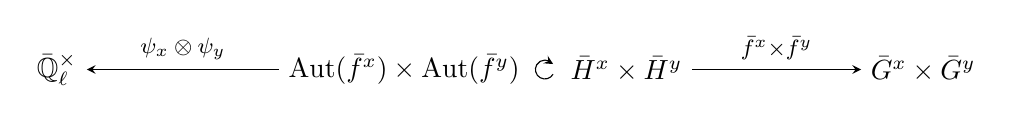
\begin{tikzpicture}[auto,style={rectangle}]
  \node (0) at (0,0) {$\EEx$};
  \node (1) [anchor=east] at (6,0) {$\Aut(\bf^x) \times \Aut(\bf^y)$};
  \node (2) [anchor=west] at (6.4,0) {$\bH^x \times \bH^y$};
  \node (3) at (11,0) {$\bG^x \times \bG^y$};
  \draw [->] (1) to node[swap, label] {$\psi_x \otimes \psi_y$} (0);
  \draw [->] (6.3,-0.06) arc (330:40:0.12) -- (6.3,0.07);
  \draw [->] (2) to node[label] {$\bf^x \tight{0}{\times}{0} \bf^y$} (3);
  \end{tikzpicture}
  \]
  On the other hand, the diagram for the local system $\bm_{x,y}^* \gcs{L}^{x+y}$
  is found by pulling-back the diagram for $\gcs{L}^{x+y}$ along
  $\bm_{x,y} : \bH^x\times\bH^y \to \bH^{x+y}$;
  the result is the middle horizontal diagram below, where we use the
  fact that the covering group of the middle arrow is $\Aut(\bf^{x+y})$, canonically.
  
  \vspace{0.2in}
  
  \[
  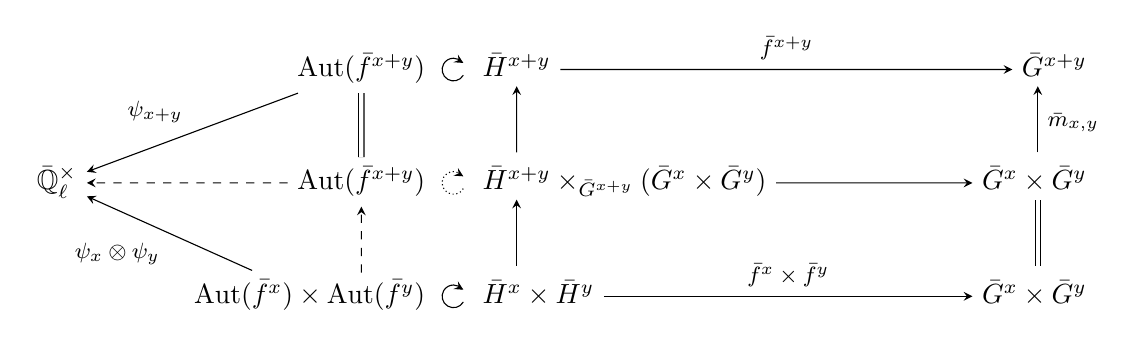
\begin{tikzpicture}[auto,style={shape={asymmetrical rectangle}},scale=1.2]
  \node (12) [anchor=east] at (4,2.4) {$\Aut(\bf^{x+y})$};
  \node (22) [anchor=west] at (4.4,2.4) {$\bH^{x+y}$};
  \node (32) [anchor=east] at (11,2.4) {$\bG^{x+y}$};
  \node (01) at (0,1.2) {$\EEx$};
  \node (11) [anchor=east] at (4,1.2) {$\Aut(\bf^{x+y})$};
  \node (21) [anchor=west] at (4.4,1.2) {$\bH^{x+y} \times_{\bG^{x+y}} (\bG^x\times\bG^y)$};
  \node (31) [anchor=east] at (11,1.2) {$\bG^x\times \bG^y$};
  \node (10) [anchor=east] at (4,0) {$\Aut(\bf^x)\times \Aut(\bf^y)$};
  \node (20) [anchor=west] at (4.4,0) {$\bH^x\times \bH^y$};
  \node (30) [anchor=east] at (11,0) {$\bG^x\times \bG^y$};
  \draw [->] (4.3,2.34) arc (330:40:0.12) -- (4.3,2.47);
  \draw [->, densely dotted] (4.3,1.14) arc (330:40:0.12) -- (4.3,1.27);
  \draw [->] (4.3,-0.06) arc (330:40:0.12) -- (4.3,0.07);
  \draw [->] (12) to node[swap,label] {$\psi_{x+y}$} (01);
  \draw [->, dashed] (11) -- (01);
  \draw [->] (10) to node[label] {$\psi_x \otimes \psi_y$} (01);
  \draw [->, dashed] ($(11.south) + (0,-0.7)$) -- (11);
  \draw [double equal sign distance] (11) -- (12);
  \draw [->] (22) to node[label] {$\bf^{x+y}$} (32);
  \draw [->] ($(22.south) + (0,-0.7)$) -- (22);
  \draw [->] (21) -- (31);
  \draw [->] ($(32.225) + (0,-0.7)$) to node[swap] {\footnotesize{$\bm_{x,y}$}} (32.225);
  \draw [->] ($(22.south) + (0,-1.9)$) -- ($(22.south) + (0,-1.2)$);
  \draw [->] (20) to node[label] {$\bf^x \times \bf^y$} (30);
  \draw [double equal sign distance] ($(32.225) + (0,-1.9)$) -- ($(32.225) + (0,-1.2)$);
  \end{tikzpicture}
  \]
  Now, the homomorphism from the covering group of
  $\bf^x\times\bf^y$ to the covering group of
  $\bf^{x+y}$ induced by the composition
  $ \bH^x\times \bH^y \to \bH^{x+y} \times_{\bG^x\times\bG^y} \bG^x\times\bG^y \to \bH^{x+y}$
  is precisely $(\bm_x(a),\bm_y(b)) \mapsto \bm_{x+y}(ab)$.
  Since this map commutes with the characters $\psi_x\otimes\psi_y$
  and $\psi_{x+y}$ (so, the far-left triangle commutes in the diagram above)
  it follows that, for each $x,y\in X$ the diagram above defines a canonical isomorphism
  $\mu_{x,y} : \bm_{x,y}^* \gcs{L}^{x+y} \to \gcs{L}^x \boxtimes\gcs{L}^y$.
  This defines $\mu: \bm^* \gcs{L} \iso \LxL$.
  It is straightforward (but laborious) to show that the pair
  $(\gcs{L},\mu)$ satisfies condition \ref{CS.1}.

  Now we turn to the definition of $\phi : \Frob{G}^* \gcs{L} \to \gcs{L}$.
  As above, we define this isomorphism through a family of
  isomorphisms on the connected components of $\bG$. The
  restriction of $\Frob{G}$ to $\bG^x$ defines an isomorphism
  $\Frob{G}^x : \bG^x \to \bG^{\Frob{\Fq}(x)}$.
  %\[
  %\xymatrix{
  %\ar[d]_{\Frob_x} \bG^x \ar[r] & \ar[d]_{\Frob{G}} \bG\\
  %\bG^{\Frob{\Fq}(x)} \ar[r] & \bG\\
  %}
  %\]
  Pull back the finite etale covering in the diagram for
  $\gcs{L}^{\Frob{\Fq}(x)}$ along $\Frob{G}^x$ and compare the result with the
  finite etale covering in the diagram for $\gcs{L}^{x}$.

  \[
  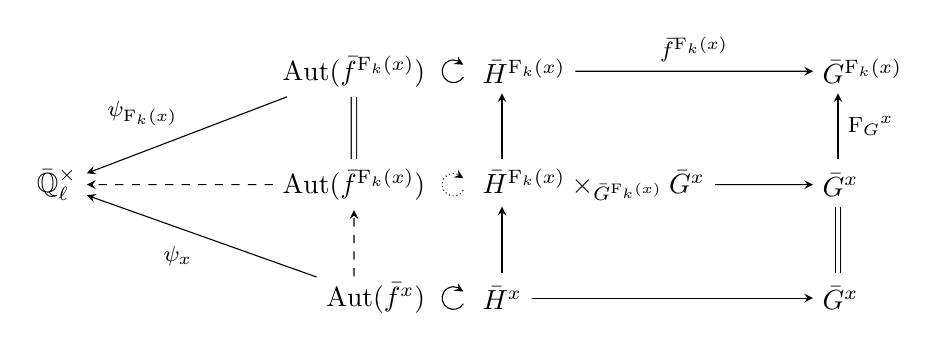
\begin{tikzpicture}[auto,style={rectangle},scale=1.2]
  \node (12) [anchor=east] at (4,2.4) {$\Aut(\bf^{\Frob{\Fq}(x)})$};
  \node (22) [anchor=west] at (4.4,2.4) {$\bH^{\Frob{\Fq}(x)}$};
  \node (32) [anchor=west] at (8,2.4) {$\bG^{\Frob{\Fq}(x)}$};
  \node (01) at (0,1.2) {$\EEx$};
  \node (11) [anchor=east] at (4,1.2) {$\Aut(\bf^{\Frob{\Fq}(x)})$};
  \node (21) [anchor=west] at (4.4,1.2) {$\bH^{\Frob{\Fq}(x)} \times_{\bG^{\Frob{\Fq}(x)}} \bG^x$};
  \node (31) [anchor=west] at (8,1.2) {$\bG^x$};
  \node (10) [anchor=east] at (4,0) {$\Aut(\bf^x)$};
  \node (20) [anchor=west] at (4.4,0) {$\bH^x$};
  \node (30) [anchor=west] at (8,0) {$\bG^x$};
  \draw [->] (4.3,2.34) arc (330:40:0.12) -- (4.3,2.47);
  \draw [->, densely dotted] (4.3,1.14) arc (330:40:0.12) -- (4.3,1.27);
  \draw [->] (4.3,-0.06) arc (330:40:0.12) -- (4.3,0.07);
  \draw [->] (12) to node[swap,label] {$\psi_{\Frob{\Fq}(x)}$} (01);
  \draw [->, dashed] (11) -- (01);
  \draw [->] (10) to node[label] {$\psi_x$} (01);
  \draw [->, dashed] ($(11.south) + (0,-0.7)$) -- (11);
  \draw [double equal sign distance] (11) -- (12);
  \draw [->] (22) to node[label] {$\bf^{\Frob{\Fq}(x)}$} (32);
  \draw [->] ($(22.225) + (0,-0.7)$) -- (22.225);
  \draw [->] (21) -- (31);
  \draw [->] ($(32.222) + (0,-0.7)$) to node[swap] {\footnotesize{$\Frob{G}^x$}} (32.222);
  \draw [->] ($(22.225) + (0,-1.9)$) -- ($(22.225) + (0,-1.2)$);
  \draw [->] (20) -- (30);
  \draw [double equal sign distance] ($(32.222) + (0,-1.9)$) -- ($(32.222) + (0,-1.2)$);
  \end{tikzpicture}
  \]
  The covering group of $\bH^{\Frob{\Fq}(x)} \times_{\bG^{\Frob{\Fq}(x)}} \bG^x$
  is isomorphic to $\Aut(\bf^{\Frob{\Fq}(x)})$, canonically, so
  $(\Frob{G}^x)^* \gcs{L}^{\Frob{\Fq}(x)}$ is defined by the middle (horizontal)
  diagram, above.  We define the sheaf homomorphism
  $\phi_x : (\Frob{G}^x)^* \gcs{L}^{\Frob{\Fq}(x)} \to \gcs{L}^x$ by the canonical morphism
  $\bH^x \to \bH^{\Frob{\Fq}(x)} \times_{\bG^{\Frob{\Fq}(x)}} \bG^x \to $;
  to see that this defines a sheaf homomorphism it is sufficient to
  check that the character $\psi_x$ commutes with the family of isomorphisms
  $\phi_x : (\Frob{G}^* \gcs{L})\vert_{\bG^x} \iso (\Frob{G}^x)^* \gcs{L}^{\Frob{x}} \to \gcs{L}^x$
  now defines the isomorphism $\phi : \Frob{G}^* \gcs{L} \to \gcs{L}$.
  \Clifton{Add some detail here.}
  This isomorphism is compatible with $\mu$ in the sense of condition~\ref{CS.2}.
\end{proof}
\Clifton{I can flesh out this remark once I've promoted the definition of $\GCb(G)$ (category of bounded geometrized characters on $G$).}
\begin{remark}
  We have seen that if $f : H\to G$ is a finite etale cover of $G$ by
  a smooth group scheme and if all geometric automorphisms of $f$ are
  fixed by Frobenius, then every character of $\ker f$ determines a
  geometrized character on $G$. However, it is not true that every character
  sheaf on $G$ arises in this manner.
\end{remark}

%\input{centralextensions}

\section{Main result regarding geometrized characters}

%\input{snake}
\begin{theorem}\label{thm:snake}
  If $G$ is a smooth abelian group scheme, locally of finite type over
  $\Fq$, and the abelian group $\pi_0(G)(\bFq)$ (the geometric
  component group) is finitely generated, then the trace of Frobenius
  homomorphism
  \[
  \trFrob{G} : \GCiso{G} \to \Hom_\text{grp}(G(\Fq),\EEx),
  \]
  from the Picard group of the category of geometrized characters on $G$ to
  the group of characters of $G(\Fq)$, is an isomorphism.
\end{theorem}

\begin{proof}
  Consider the short exact sequence in the category of smooth group
  schemes, locally of finite type over $\Fq$, defining the component
  group scheme for $G$:
  \begin{equation}\label{eq:pi0}
  \begin{tikzcd}
    1 \rar & G^0 \rar & G \rar & \pi_0(G) \rar & 0.
  \end{tikzcd}
  \end{equation}
  Let
  \[
  \begin{tikzcd}[row sep=30]
    {}& \ker t_{\pi_0(G)} \dar & \arrow[dashed]{d} \ker \trFrob{G} & \ker t_{G^0} \dar & \\
    0 \rar & \GCiso{\pi_0(G)} \rar \dar{t_{\pi_0(G)}}
    & \GCiso{G} \rar \dar{\trFrob{G}} & \GCiso{G^0} \rar \dar{t_{G^0}} & 0\\
    0 \rar & \Hom(\pi_0(G)(\Fq),\EEx) \rar \dar
    & \arrow[dashed]{d} \Hom(G(\Fq),\EEx) \rar & \Hom(G^0(\Fq),\EEx) \rar \dar & 0\\
    & \coker t_{\pi_0(G)} & \coker \trFrob{G} &  \coker t_{G^0} &
  \end{tikzcd}
  \]
  be the commutative diagram of abelian groups obtained by applying
  Proposition~\ref{prop:pullback} to \eqref{eq:pi0}.  By
  Proposition~\ref{prop:connected}, $\ker t_{G^0} =0$ and $\coker t_{G^0}=0$.
  By Propositions~\ref{prop:etale} and \ref{prop:X}, $\ker t_{\pi_0(G)}=0$
  and $\coker t_{\pi_0(G)}=0$.

  The sequence of character groups is left-exact: by
  Proposition~\ref{prop:pullback}, it is dual to the exact sequence of
  abelian groups
  \begin{equation}\label{eq:pi1}
  \begin{tikzcd}
    1 \rar & G^0(\Fq) \rar & G(\Fq) \rar & \pi_0(G)(\Fq) \rar & 0;
  \end{tikzcd}
  \end{equation}
  since $\Hom(\ - \ ,\EEx)$ is left-exact, the sequence of
  character groups is left exact.

  The sequence of Picard groups is right-exact: it is exact at
  $\GCiso{G^0}$ by Proposition~\ref{prop:restriction}; and
  it is exact at $\GCiso{G}$ because the left-square
  commutes (by Proposition~\ref{prop:pullback}), the bottom sequence
  is exact at $\Hom(G(\Fq),\EEx)$ and $\coker t_{\pi_0(G)} =0$
  (by Propositions~\ref{prop:etale} and \ref{prop:X}) and
  \[
  \image(\GCiso{\pi_0(G)} \to \GCiso{G}) \subseteq \ker(\GCiso{G} \to \GCiso{G^0}),
  \]
  by the last part of Proposition~\ref{prop:pullback}. Specifically,
  suppose $\cs{L}$ is a geometrized character on $G$ that is trivial on
  $G^0$. Then $\trFrob{\cs{L}}\vert_{G^0(\Fq)} = \trFrob{\cs{L}^0} =0$,
  by Proposition~\ref{prop:pullback} again. Since the sequence of
  character groups is exact at $\Hom(G(\Fq),\EEx)$, there is
  some $\chi \in \Hom(\pi_0(G)(\Fq),\EEx)$ such that the
  pull-back of $\chi$ along $G(\Fq)\to \pi_0(G)(\Fq)$ is
  $\trFrob{\cs{L}}$. By Propositions~\ref{prop:etale} and \ref{prop:X},
  there is a a geometrized character $\cs{L}_\chi$ on $\pi_0(G)$, unique up
  to isomorphism, such that $\trFrob{\cs{L}_\chi} = \chi$. By
  Proposition~\ref{prop:pullback} again, $\cs{L}$ is isomorphic to the
  image of $\cs{L}_\chi$ under the monoidal functor $\GC(\pi_0(G)) \to \GC(G)$.

  It now follows immediately from the snake lemma that $\trFrob{G}$ is an
  isomorphism of groups.
\end{proof}

\section{Application to characters of bounded depth}

%\input{GdeN}
Let $p$ be a prime number. Let $K$ be a local field with residue field
$\Fq$, where $p$ divides $q$. Let $\OK$ be the ring of integers of $K$
and let $\pK$ be the maximal ideal in $\OK$.
%
In this section we introduce a group scheme $\GN{T}$ over $\Fq$
obtained by applying the Greenberg functor to the N\'eron lft-model
for $T$ and establish some basic facts about $\GN{T}$

%\subsection{The N\'eron locally finite type model for $T$}

The lft-N\'eron model for $T$, denoted here by $\TT$, is a separated,
smooth, commutative group scheme locally of finite type over $\OK$
with generic fibre $T$, that enjoys the N\'eron mapping property: if
$X$ is a smooth scheme over $\OK$ then every morphism $X_\eta \to T$
over $K$ extends uniquely to a morphism $X \to \TT$. Equivalently, the
N\'eron mapping property states that the function
$\Hom_{\OK} (X,\TT) \to \Hom_K(X_\eta,T)$, given by restriction to
generic fibres, is a bijection; in particular, this implies $\TT(\OK) = T(K)$.

For each $d\in \ZZ_{>0}$, let $\TT_{d}$ be the smooth group scheme over
$\OK/\pK^d$ obtained from $\TT$ by base change along $\OK \to
\OK/\pK^d$. Observe that $\OK/\pK^d$ is an Artin ring and
$\TT_{d}$ is locally of finite type over $\OK/\pK^d$.

Let $\GN{T}_{d} = \Gr(\TT_d)$ be the group scheme over $\Fq$ produced by applying
the Greenberg functor to $\TT_{d}$. (See \cite{Greenberg:2} and
\cite[Ch. 9, \S 6]{BLR} for background on the Greenberg functor.)
%Then $\GN{T}_d(\Fq) = \TT(\OK/\pK^d)$.

\begin{proposition}\label{prop:GN}
  Fundamental properties of the group $\Fq$-scheme $\GN{T}_d$, for all $d\in \NN$:
  \begin{enumerate}
  \labitem{(GNd.0)}{GN0} $\GN{T}_d^0$, the identity component of
    $\GN{T}_d$, is a commutative algebraic group over $\Fq$;
  \labitem{(GNd.1)}{GNd} $\GN{T}_d$ is smooth and locally of finite type over $\Fq$;
  \labitem{(GNd.2)}{pi0} $\pi_0(\GN{T}_d) = \pi_0(\TT) \times_{\Spec{\OK}} \Spec{\Fq}$;
  \labitem{(GNd.3)}{fg} the component group of $\GN{T}_d$ is geometrically finitely generated;
  \labitem{(GNd.4)}{dFq} $\GN{T}_d(\Fq) = \TT(\OK/\pK^d)$, canonically;
\end{enumerate}
\end{proposition}

\begin{proof}
\Clifton{Proofs still missing, but all straightforward. I'll cite as much as I can, here.}
\end{proof}

%\input{application}
\begin{theorem}\label{thm:application}
  Let $T$ be an algebraic torus over a non-Archimedean local field $K$.
  Let $\GN{T}_d$ and $\GN{T}$ be as above.  For each $d \in \ZZ_{>0}$, the
  Picard group of the category of geometrized characters on $\GN{T}_d$ is
  canonically isomorphic to the group of characters of $T(K)$ of depth
  less than $d$:
  \[
  \GCiso{\GN{T}_d} \iso \Hom_{< d}(T(K),\EEx).
  \]
\end{theorem}

\begin{proof}
  By \ref{GNd} and \ref{fg}, we may apply Theorem~\ref{thm:snake} to
  $\GN{T}_d$ which provides a canonical isomorphism
  \[
  \GCiso{\GN{T}_d} \iso \Hom(\GN{T}_d(\Fq),\EEx).
  \]
  By \ref{dFq}, $\GN{T}_d(\Fq) \iso \TT(\OK/\pK^d)$ canonically.
  To finish the proof we recall that the filtration of $T(K)$ used to
  define depth has the property that $\TT(\OK/\pK^d) \cong T(K) / T(K)_d$
  \cite[Prop 5.2]{Yu} for $d \in \ZZ_{>0}$.  Thus characters of $\GN{T}_d(\Fq)$ are
  in bijection with characters of $T(K)$ vanishing on $T(K)_d$.
\end{proof}

\section{Application to admissible characters}

%\input{pro}
To conclude the paper we offer an interpretation of
Theorem~\ref{thm:application} that makes no mention of depth.

\Clifton{Explain what happens as $d$ varies.}
Suppose $d\leq d'$.

We may now assemble the group $\Fq$-schemes $\TT_{d}$ into one
glorious group pro-scheme over $\Fq$:
\begin{equation}\label{projlim}
  \GN{T} \ceq \varprojlim_{d\in \NN} \GN{T}_{d}.
\end{equation}
This is the \cdef{Greenberg transform of the lft-N\'eron model of $T$}; we will also write $\Gr$ for this functor on $\OK$-schemes.

\Clifton{Prove that $\GN{T}$ is a scheme? Strictly speaking, we don't
  care about \ref{scheme}.}
  
\Clifton{Must still define $\GC(\GN{T})$, since it is not an instance
 of our definitions, above.}
  
\begin{proposition}
  Fundamental properties of $\GN{T}$:
  \begin{enumerate}
  \labitem{(GN.0)}{scheme} $\GN{T}$ is a commutative group scheme over $\Fq$;
  \labitem{(GN.1)}{T(K)} $\GN{T}(\Fq) = T(K)$, canonically.
  \end{enumerate}
\end{proposition}


\begin{corollary}
  \[
  \GCiso{\GN{T}} \iso \Hom_\text{ad}(T(K),\EEx)
  \]
\end{corollary}

\section{The transfer principle}

\David{We should add a discussion of why we care about the transfer principle.}
We recall the notion of $N$-congruent tori from \cite[\S 2]{CY}.  Suppose $T$ and $T'$
are tori over non-Archimedian local fields $K$ and $K'$, splitting over $L$ and $L'$ respectively.

\begin{definition}
 We say that $T$ and $T'$ are \emph{$N$-congruent} if there are isomorphisms
 \begin{align*}
  \alpha : \OL/\pi_K^N \OL &\to \OO{L'}/\pi_{K'}^N \OO{L'} \\
  \beta : \Gal(L/K) &\to \Gal(L'/K') \\
  \phi : X^*(T) &\to X^*(T')
 \end{align*}
 satisfying the following conditions:
 \begin{enumerate}
  \item $\alpha$ induces an isomorphism $\OK/\pi_K^N \OK \to \OO{K'}/\pi_{K'}^N \OO{K'}$,
  \item $\alpha$ is $\Gal(L/K)$-equivariant relative to $\beta$: $\alpha(\gamma x) = \beta(\gamma) \alpha(x)$
  for $\gamma \in \Gal(L/K)$ and $x \in \OL/\pi_K^N \OL$,
  \item $\phi$ is $\Gal(L/K)$-equivariant relative to $\beta$.
 \end{enumerate}
\end{definition}

One of the main results of \cite{CY} gives an isomorphism of group schemes between
$\TT_d$ and $\TT'_d$ assuming that $T$ and $T'$ are sufficiently congruent.
They define a quantity $h$ as the smallest integer so that $\pi^h$ lies in the
Jacobian ideal associated to a natural embedding of $T$ into an induced torus \cite[\S 8.1]{CY}.
They then prove the following theorem:

\begin{theorem}[{\cite[Thm. 8.5]{CY}}]
 Suppose that $T$ and $T'$ are $N$-congruent for $N > 3h$.  Then there is a canonical isomorphism
 \[
  \TT_{N-3h} \to \TT'_{N-3h}
 \]
 determined by $\alpha, \beta$ and $\phi$.
\end{theorem}

As an immediate consequence of this theorem and Theorem \ref{thm:application} we have the following corollary:

\begin{corollary}
 Suppose that $T$ and $T'$ are $N$-congruent for $N > 3h$.  Then there is a canonical equivalence of categories
 \[
  \GC(\GN{T}_{N-3h}) \to \GC(\GN{T}'_{N-3h})
 \]
 determined by $\alpha, \beta$ and $\phi$ inducing the isomorphism
 \[
  \Hom(T(K) / T(K)_{N-3h}, \EEx) \to \Hom(T'(K') / T'(K')_{N-3h}, \EEx)
 \]
\end{corollary}

\begin{bibdiv}
\begin{biblist}

\bib{BBD}{article}{
   author={Be{\u\i}linson, A. A.},
   author={Bernstein, J.},
   author={Deligne, P.},
   title={Faisceaux pervers},
%   language={French},
   conference={
      title={Analyse et topologie sur les espaces singuliers (I)},
      address={Luminy},
      date={1981},
   },
   book={
      series={Ast\'erisque},
      volume={100},
      publisher={Soc. Math. France},
      place={Paris},
   },
   date={1982},
%   pages={5--171},
%   review={\MR{751966 (86g:32015)}},
}

\bib{BLR}{book}{
   author={Bosch, Siegfried},
   author={L{\"u}tkebohmert, Werner},
   author={Raynaud, Michel},
   title={N\'eron models},
   series={Ergebnisse der Mathematik und ihrer Grenzgebiete (3) [Results in
   Mathematics and Related Areas (3)]},
   volume={21},
   publisher={Springer-Verlag},
   place={Berlin},
   date={1990},
%   pages={x+325},
%   isbn={3-540-50587-3},
%   review={\MR{1045822 (91i:14034)}},
}

\bib{Brandal}{book}{
 author={Brandal, Willy},
 title={Commutative Rings whose Finitely Generated Modules Decompose},
 publisher={Springer-Verlag},
 date={1979},
 series={Lecture Notes in Mathematics}
 number={723}
}

\bib{Chai}{article}{
   author={Chai, C.L.},
   title={N\'eron models for semiabelian varieties: congruence and change of base field.},
   journal={Asian J. Math.},
   volume={4},
   number={4},
   date={2000},
   pages={715--736}}
   
\bib{CY}{article}{
   author={Chai, C.L.},
   author={Yu, J.-K.},
   title={Congruences of N\'eron models for tori and the Artin conductor},
   journal={Ann. of Math.},
   volume={154},
   number={2},
   date={2001},
   pages={347-382}}

\bib{Deligne:tensorielles}{article}{
   author={Deligne, P.},
   title={Cat\'egories tensorielles},
%   language={French, with English summary},
%   note={à Yu. I. Manin, en témoignage d'admiration},
   journal={Mosc. Math. J.},
   volume={2},
   date={2002},
   number={2},
   pages={227--248},
%   issn={1609-3321},
%   review={\MR{1944506 (2003k:18010)}},
}

\bib{Deligne:Weil2}{article}{
   author={Deligne, Pierre},
   title={La conjecture de Weil. II},
%   language={French},
   journal={Inst. Hautes \'Etudes Sci. Publ. Math.},
   number={52},
   date={1980},
   pages={137--252},
%   issn={0073-8301},
%   review={\MR{601520 (83c:14017)}},
}

\bib{Greenberg:2}{article}{
   author={Greenberg, Marvin J.},
   title={Schemata over local rings. II},
   journal={Ann. of Math. (2)},
   volume={78},
   date={1963},
   pages={256--266},
%   issn={0003-486X},
%   review={\MR{0156855 (28 \#98)}},
}

\bib{SGA1a}{book}{
   author={Grothendieck, Alexander},
   title={Rev\^etements \'etales et groupe fondamental. Fasc. I: Expos\'es 1
   \`a 5},
   series={S\'eminaire de G\'eom\'etrie Alg\'ebrique},
   volume={1960/61},
   publisher={Institut des Hautes \'Etudes Scientifiques},
   place={Paris},
   date={1963},
%   pages={iv+143 pp. (not consecutively paged) (loose errata)},
%   review={\MR{0217087 (36 \#179a)}},
}

\bib{Kamgarpour}{article}{
   author={Kamgarpour, Masoud},
   title={Stacky abelianization of algebraic groups},
   journal={Transform. Groups},
   volume={14},
   date={2009},
   number={4},
   pages={825--846},
%   issn={1083-4362},
%   review={\MR{2577200 (2011b:20136)}},
%   doi={10.1007/s00031-009-9067-8},
}

\bib{Laumon}{article}{
   author={Laumon, G.},
   title={Transformation de Fourier, constantes d'\'equations fonctionnelles
   et conjecture de Weil},
%   language={French},
   journal={Inst. Hautes \'Etudes Sci. Publ. Math.},
   number={65},
   date={1987},
   pages={131--210},
%   issn={0073-8301},
%   review={\MR{908218 (88g:14019)}},
}

\bib{SGA4.5}{book}{
   author={Deligne, P.},
   title={Cohomologie \'etale},
   series={Lecture Notes in Mathematics, Vol. 569},
   note={S\'eminaire de G\'eom\'etrie Alg\'ebrique du Bois-Marie 1963-64 SGA
   4$\frac{1}{2}$; 
   Avec la collaboration de J. F. Boutot, A. Grothendieck, L. Illusie et J.
   L. Verdier},
   publisher={Springer-Verlag},
   place={Berlin},
%date={4h},
   date={1977},
%   pages={iv+312pp},
%   review={\MR{0463174 (57 \#3132)}},
}

\bib{Deligne:Weil2}{article}{
   author={Deligne, Pierre},
   title={La conjecture de Weil. II},
%   language={French},
   journal={Inst. Hautes \'Etudes Sci. Publ. Math.},
   number={52},
   date={1980},
   pages={137--252},
%   issn={0073-8301},
%   review={\MR{601520 (83c:14017)}},
}

\bib{SGA7.2}{book}{
   title={Groupes de monodromie en g\'eom\'etrie alg\'ebrique. II},
%   language={French},
 author={Deligne, P.},
 author={Katz, N.},
   series={Lecture Notes in Mathematics, Vol. 340},
   note={S\'eminaire de G\'eom\'etrie Alg\'ebrique du Bois-Marie 1967--1969
   (SGA 7 II);
   Dirig\'e par P. Deligne et N. Katz},
   publisher={Springer-Verlag},
   place={Berlin},
   date={1973},
%   pages={x+438},
%   review={\MR{0354657 (50 \#7135)}},
}

\bib{Tate:thesis}{article}{
   author={Tate, J. T.},
   title={Fourier analysis in number fields, and Hecke's zeta-functions},
   conference={
      title={Algebraic Number Theory (Proc. Instructional Conf., Brighton,
      1965)},
   },
   book={
      publisher={Thompson, Washington, D.C.},
   },
   date={1967},
   pages={305--347},
   review={\MR{0217026 (36 \#121)}},
}

\bib{vdG&M}{book}{
author={van der Geer},
author={Moonen},
title={Abelian Varieties},
note={http://staff.science.uva.nl/$\sim$bmoonen/boek/BookAV.html}
}


\bib{Xarles}{article}{
   author={Xarles, Xavier},
   title={The scheme of connected components of the N\'eron model of an algebraic torus},
   journal={J. Reine Angew. Math.},
   volume={437},
   date={1993},
   pages={167--179},
%   issn={0075-4102},
%   review={\MR{1212256 (94d:14044)}},
%   doi={10.1515/crll.1993.437.167},
}


\bib{Yu}{article}{
   author={Yu, Jiu-Kang},
   title={Smooth models associated to concave functions in Bruhat-Tits theory}
}

\end{biblist}
\end{bibdiv}

\end{document}
